\documentclass[12pt]{ai_conquer2026}
\special{pdf:minorversion 7}
\addbibresource{references.bib}
\usepackage{multirow}
\usepackage{booktabs}
\usepackage{amsmath,amssymb}
\usepackage{graphicx}
\usepackage{subcaption}

% --- Brand colors for table formatting ---
\definecolor{brandIndigo}{HTML}{333D91} 
\definecolor{rowLavender}{HTML}{EEECFA}

\title{%
    \centering
    \Large {AI VIET NAM -- AI Conquer 2026 -- Topic Team}\\[.5ex]  
    \Huge \textbf{Week 03 Progress Report: Breaking the Parameter-Efficiency Wall in Vision MLPs via Hierarchical Pyramids, Structural Re-parameterization, and Local Spatial Inductive Biases}\\[.5ex]
}

\author{
    {\bfseries\large Debug Team} \\[1.2em]
    \begin{tabular}{ccc}
        Nguyễn Thị Diễm My & Lê Tiến Anh & Nguyễn Mạnh Tân \\[1.2em]
    \end{tabular}\\
    \begin{tabular}{cc}
        Hoàng Nguyễn Nhật Minh & Lê Minh Hoàng
    \end{tabular}
}
\date{}

% Header --------------------------------------------------------------------
\pagestyle{fancy}
\fancyhf{}
\lhead{\href{https://www.facebook.com/aivietnam.edu.vn}{\textcolor{aivnGreen}{\bfseries AI VIET NAM (AI Conquer 2026)}}}
\rhead{\href{https://aivietnam.edu.vn/}{\textcolor{aivnGreen}{\bfseries aivietnam.edu.vn}}}
\fancyfoot[C]{\thepage}
\renewcommand{\headrulewidth}{1.0pt}
\renewcommand{\headrule}{{\color{aivnGreen}\hrule width\headwidth height\headrulewidth \vskip-\headrulewidth}}

% Section Numbering in Arabic (1., 1.1., 1.1.1., ...)
\renewcommand{\thesection}{\arabic{section}}
\renewcommand{\thesubsection}{\thesection.\arabic{subsection}}
\renewcommand{\thesubsubsection}{\thesubsection.\arabic{subsubsection}}
\titleformat{\section}{\normalfont\LARGE\bfseries}{\thesection.}{0.6em}{}
\titleformat{\subsection}{\normalfont\large\bfseries}{\thesubsection.}{0.5em}{}
\titleformat{\subsubsection}{\normalfont\normalsize\bfseries}{\thesubsubsection.}{0.4em}{}

% Ensure English labels throughout the document
\selectlanguage{english}
\addto\captionsenglish{%
    \renewcommand{\tablename}{Table}%
    \renewcommand{\figurename}{Figure}%
    \renewcommand{\contentsname}{Table of Contents}%
    \renewcommand{\abstractname}{Abstract}%
    \renewcommand{\refname}{References}%
}
\AtBeginDocument{%
    \selectlanguage{english}%
    \renewcommand{\tablename}{Table}%
    \renewcommand{\figurename}{Figure}%
    \renewcommand{\contentsname}{Table of Contents}%
    \renewcommand{\abstractname}{Abstract}%
}

% Float layout and whitespace tightening
\makeatletter
\setlength{\@fptop}{0pt}
\setlength{\@fpsep}{12pt plus 2pt minus 2pt}
\setlength{\@fpbot}{0pt plus 1fil}
\makeatother

\raggedbottom

\renewcommand{\topfraction}{0.95}
\renewcommand{\bottomfraction}{0.95}
\renewcommand{\textfraction}{0.05}
\renewcommand{\floatpagefraction}{0.75}
\setlength{\floatsep}{10pt plus 2pt minus 2pt}
\setlength{\textfloatsep}{12pt plus 2pt minus 2pt}
\setlength{\intextsep}{10pt plus 2pt minus 2pt}

\begin{document}
\maketitle

\addvspace{-2.5em}
\setlength{\epigraphwidth}{0.6\textwidth}

\begin{abstract}
In our Week 02 benchmark on CIFAR-100, standard columnar vision MLPs such as ResMLP suffered from severe parameter inefficiency, requiring over 2.19 million parameters to attain a modest 62.40\% Top-1 validation accuracy. This limitation stemmed from the lack of hierarchical multi-scale feature downsampling and absent spatial inductive biases. In Week 03, our team investigated four architectural solutions to overcome this bottleneck:
\begin{itemize}
    \item \textbf{Pyramid-ResMLP and Pyramid-ResMLP Pure:} A 3-stage hierarchical architecture replacing columnar patch extraction with overlapping convolution stems and progressive token downsampling. In Pyramid-ResMLP, structural re-parameterization (RepTokenMix layer) injects local depthwise convolutions during training and collapses them into a single linear projection for deployment. Pyramid-ResMLP Pure serves as an ablation control with unaugmented linear mixing.
    \item \textbf{Shift-ResMLP:} A parameter-free spatial communication scheme that routes features through 4-direction coordinate channel shifts, eliminating all spatial matrix parameters.
    \item \textbf{CA-Mixer:} A Neural Cellular Automata (NCA) mixer with fixed perception operators that enables resolution-agnostic spatial mixing with strictly constant parameter counts.
    \item \textbf{MetaFormer and HybridFormer:} Explorations into non-parametric pooling and hybrid early-pooling / late-attention designs.
\end{itemize}

Empirical evaluations demonstrate substantial breakthroughs. On CIFAR-100, Pyramid-ResMLP achieves \textbf{72.18\%} Top-1 validation accuracy with only \textbf{1.79M deployable parameters} and a rapid \textbf{44.53-minute} training time, surpassing the Week 02 RepMLP baseline (71.46\% in 107.13 minutes with 2.16M parameters) while using 217k fewer parameters. Our ablation with Pyramid-ResMLP Pure (68.22\%) reveals a distinct two-step progression: $+5.82\%$ from hierarchical downsampling, followed by $+3.96\%$ from structural re-parameterization. Meanwhile, Shift-ResMLP reaches \textbf{72.92\%} without any learnable spatial weights, and CA-Mixer delivers \textbf{62.87\%} with 1.21M parameters across variable resolutions. Finally, scaling Pyramid-ResMLP to Tiny-ImageNet ($64*64$) yields \textbf{62.93\%} Top-1 accuracy with DropPath regularization. These results demonstrate that hierarchical token reduction combined with localized spatial routing resolves the parameter-efficiency dilemma of vision MLPs.
\end{abstract}


\newpage
\setcounter{tocdepth}{2}
\tableofcontents
\thispagestyle{fancy}

\newpage
\section{Overview and Problem Formulation}
\label{section:overview}

\subsection{Motivation: Addressing the Parameter-Efficiency Bottleneck in ResMLP}
At the conclusion of our Week 02 benchmark, our team identified a fundamental structural limitation in columnar vision MLP architectures. Under identical experimental conditions on CIFAR-100, vanilla ResMLP~\cite{touvron2021resmlp} required 2,191,204 parameters to achieve a Top-1 validation accuracy of 62.40\%. In contrast, modern hierarchical architectures such as PoolFormer~\cite{yu2022metaformer} and RepMLP~\cite{ding2022repmlp} demonstrated substantially higher accuracy with equal or fewer parameters.

This performance gap raised an important research question: \textit{Why does columnar ResMLP struggle to learn efficient visual representations from small datasets, and why do hierarchical architectures achieve significantly higher parameter efficiency?}

Our team formulated the working hypothesis that isotropic columnar models suffer from two structural disadvantages:
\begin{itemize}
    \item \textbf{Absence of multi-scale feature hierarchies:} In vanilla ResMLP, non-overlapping patch slicing maintains a rigid, single-scale token sequence ($N = 64$ for patch size $P = 4$) throughout all network layers. Because spatial token dimensions never contract, early layers are forced to process global token interactions prematurely, while later layers lack compact, semantically rich spatial representations.
    \item \textbf{Lack of 2D translation equivariance:} A dense linear token mixing matrix $\mathbf{W} \in \mathbb{R}^{N \times N}$ treats all spatial positions as arbitrary permutation-invariant tokens. It does not possess any built-in concept of adjacent 2D pixel proximity, requiring massive training data or heavy regularizations to learn spatial relationships from scratch.
\end{itemize}

We hypothesized that introducing convolutional patch downsampling (a pyramid backbone) before each stage shrinks the token sequence, broadens the effective receptive field, and provides strong multi-scale inductive bias, enabling the network to achieve high accuracy with a fraction of the parameter cost.

\subsection{Research Objectives for Week 03}
To verify this hypothesis and explore the broader design space of spatial mixing, our team conducted five complementary research investigations in Week 03:
\begin{itemize}
    \item \textbf{a. Validating hierarchical pyramids with re-parameterization:} We developed Pyramid-ResMLP, which integrates an overlapping convolution stem, a 3-stage feature pyramid ($16 \times 16 \rightarrow 8 \times 8 \rightarrow 4 \times 4$ token resolution for the $32 \times 32$ CIFAR-100 dataset), and a structural re-parameterization token mixer (RepTokenMix layer). To isolate the exact source of performance gains, we also trained Pyramid-ResMLP Pure as an unaugmented ablation control.
    \item \textbf{b. Evaluating parameter-free spatial communication:} We evaluated Shift-ResMLP, which replaces matrix multiplication in token mixing with a 4-direction coordinate channel shift. This eliminates all learnable spatial weights, providing an empirical test of whether non-parametric coordinate routing can provide sufficient inductive bias.
    \item \textbf{c. Resolution-agnostic cellular automata mixing:} We explored CA-Mixer, which replaces fixed-dimension matrix mixing with Neural Cellular Automata (NCA) updates. Because its perception operators are local 2D convolutions, its parameter count remains constant across arbitrary input resolutions.
    \item \textbf{d. MetaFormer and hybrid paradigms:} We examined non-parametric average pooling (PoolFormer-S12) and a hybrid architecture (HybridFormer) combining early-stage pooling with late-stage self-attention on CIFAR-100.
    \item \textbf{e. Scaling to Tiny-ImageNet ($64 \times 64$):} We evaluated whether the multi-stage pyramid design scales effectively from CIFAR-100 to Tiny-ImageNet (200 classes) under different channel capacities and regularization schedules.
\end{itemize}


\section{Architectural Design and Parameter Formulations}
\label{section:architecture}

This section details the architectural designs, mathematical formulations, and parameter breakdowns for the models investigated in Week 03. All parameter counts are computed directly from tensor layer shapes using standard multiplication without external citations.

\subsection{Pyramid-ResMLP and Pyramid-ResMLP Pure}
\label{subsection:pyramid_resmlp}

Pyramid-ResMLP is a hierarchical MLP-style architecture composed of RepTokenMix blocks and convolutional downsampling stages (Figure~\ref{fig:pyramid_resmlp_arch}). Unlike isotropic columnar MLPs that preserve fixed token sequences across all layers, Pyramid-ResMLP progressively contracts spatial dimensions while expanding channel capacity. We first present the components of the RepTokenMix block and its re-parameterization mechanism in Section~\ref{subsubsection:reptokenmix_components}, describe the overall multi-stage hierarchical architecture in Section~\ref{subsubsection:pyramid_macro}, introduce the PureTokenMix ablation control in Section~\ref{subsubsection:pure_ablation}, and derive the parameter counts in Section~\ref{subsubsection:pyramid_params}.

\begin{figure}[htbp]
\centering
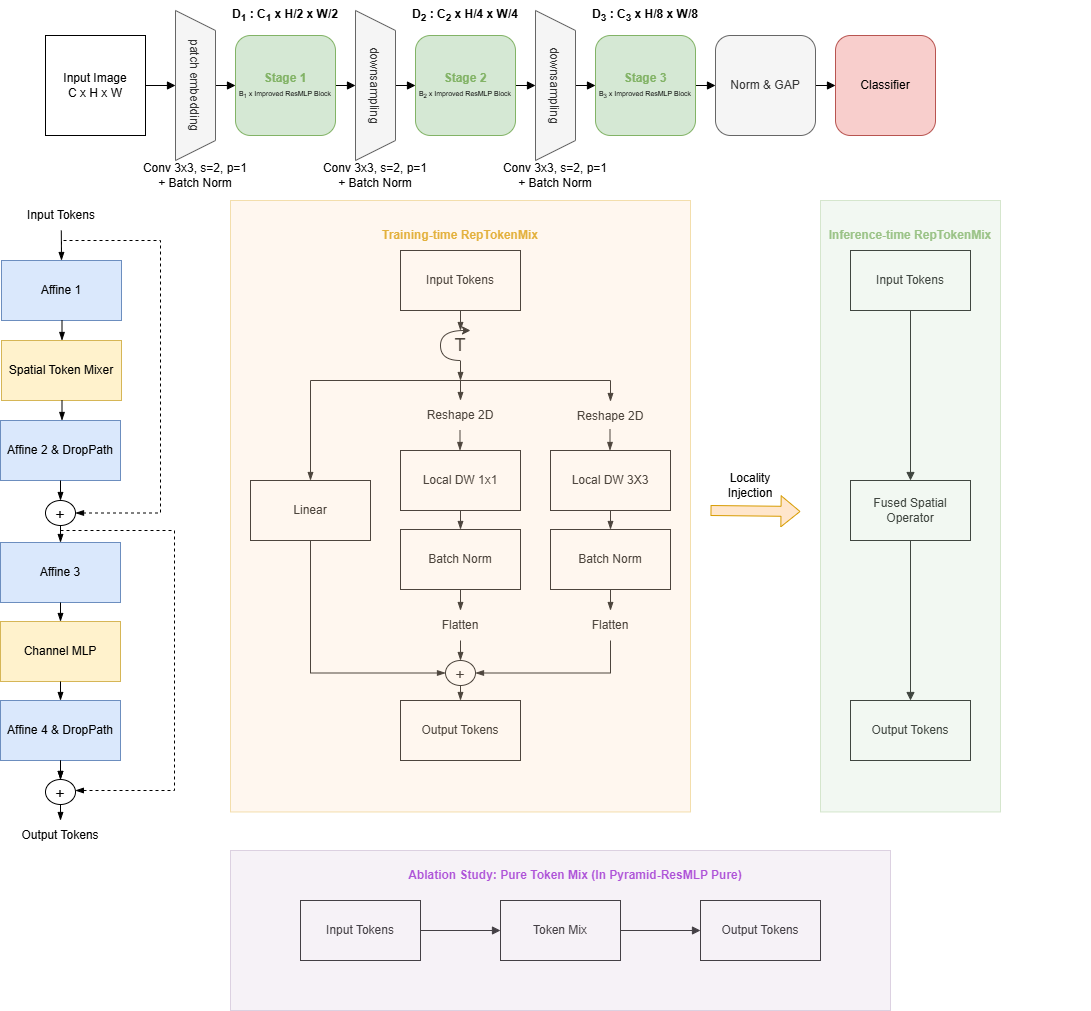
\includegraphics[width=\textwidth]{figures/pyramid_resmlp_and_pure_arch.png}
\caption{Architectural diagrams of Pyramid-ResMLP and Pyramid-ResMLP Pure: 3-stage hierarchical downsampling backbone, training-time re-parameterization in RepTokenMix block, deployment-time locality injection, and the pure linear ablation mixer.}
\label{fig:pyramid_resmlp_arch}
\end{figure}

\subsubsection{Components of RepTokenMix Block}
\label{subsubsection:reptokenmix_components}

A training-time RepTokenMix block is composed of three parallel spatial branches designed to capture multi-scale spatial dependencies: a Global Linear branch, a Local $1*1$ Depthwise Convolution branch, and a Local $3*3$ Depthwise Convolution branch, followed by channel-wise transformation layers (Figure~\ref{fig:pyramid_resmlp_arch}). The outputs of the three spatial components are combined to obtain a comprehensive transformation of the input features before channel mixing.

\textbf{Global linear branch} models long-range, cross-patch spatial dependencies across all $N_i$ token locations simultaneously. Given a sequence of tokens $\mathbf{x} \in \mathbb{R}^{B \times N_i \times C_i}$, the linear branch applies a dense weight matrix $\mathbf{W}_{\text{linear}} \in \mathbb{R}^{N_i \times N_i}$ directly along the transposed token dimension:
\begin{equation}
\mathbf{y}_{\text{linear}} = \mathbf{W}_{\text{linear}} \mathbf{x} + \mathbf{b}_{\text{linear}}.
\end{equation}
While this dense mapping allows any pair of spatial locations to exchange information in a single forward step, it treats all token coordinates as arbitrary permutation-invariant elements, discarding 2D geometric proximity.

\textbf{Local depthwise convolution branches} inject 2D translational equivariance and local spatial inductive bias without cross-channel parameter inflation. In parallel with the global linear branch, the intermediate token sequence is reshaped into a 2D spatial feature map $\mathbf{X} \in \mathbb{R}^{B \times C_i \times H_i \times W_i}$ (where $H_i * W_i = N_i$) and passed through two depthwise convolutional pathways: a $1*1$ depthwise convolution ($\text{Conv2d}(C_i, C_i, k=1, s=1, \text{groups}=C_i) + \text{BN}$) and a $3*3$ depthwise convolution ($\text{Conv2d}(C_i, C_i, k=3, s=1, p=1, \text{groups}=C_i) + \text{BN}$). Because depthwise convolutions apply independent spatial filters within each individual channel, they efficiently capture local edge continuity and adjacent pixel textures. Their outputs are flattened back into $(B, N_i, C_i)$ and combined with the linear projection:
\begin{equation}
\mathbf{y}_{\text{spatial}} = \mathbf{y}_{\text{linear}} + \text{BN}\big(\text{DWConv}_{1\times1}(\mathbf{X})\big) + \text{BN}\big(\text{DWConv}_{3\times3}(\mathbf{X})\big).
\end{equation}

\textbf{Inference-time structural re-parameterization} fuses the parallel convolution and batch normalization branches directly into the weights and biases of a single linear layer upon deployment, achieving zero-overhead locality injection. Because depthwise convolutions and batch normalizations are linear operations with respect to the input tensor, a $3*3$ depthwise convolution acts as a banded, doubly Toeplitz matrix on the flattened token sequence. By passing standard one-hot impulse tensors through the convolution and normalization paths, we extract their exact equivalent matrix transformations $\mathbf{W}_{\text{conv1x1}}, \mathbf{W}_{\text{conv3x3}} \in \mathbb{R}^{N_i \times N_i}$ and bias vectors $\mathbf{b}_{\text{conv1x1}}, \mathbf{b}_{\text{conv3x3}} \in \mathbb{R}^{N_i}$. The final deployed linear mixer is constructed as:
\begin{equation}
\mathbf{W}_{\text{fused}} = \mathbf{W}_{\text{linear}} + \mathbf{W}_{\text{conv1x1}} + \mathbf{W}_{\text{conv3x3}}, \quad \mathbf{b}_{\text{fused}} = \mathbf{b}_{\text{linear}} + \mathbf{b}_{\text{conv1x1}} + \mathbf{b}_{\text{conv3x3}}.
\end{equation}
After fusion, all parallel convolutional branches and batch normalizations are discarded. The deployed network runs as a single dense matrix multiplication $\mathbf{y} = \mathbf{W}_{\text{fused}} \mathbf{x} + \mathbf{b}_{\text{fused}}$, introducing \textbf{zero extra parameters, zero added FLOPs, and zero kernel-launch latency}.

\textbf{Channel MLP and LayerScale} perform cross-channel feature transformations following spatial token mixing. Each block contains two residual sub-layers:
\begin{equation}
\mathbf{x} \leftarrow \mathbf{x} + \text{DropPath}\Big(\boldsymbol{\gamma}_1 \odot \text{TokenMix}\big(\text{Affine}_1(\mathbf{x})\big)\Big),
\end{equation}
\begin{equation}
\mathbf{x} \leftarrow \mathbf{x} + \text{DropPath}\Big(\boldsymbol{\gamma}_2 \odot \text{ChannelMLP}\big(\text{Affine}_2(\mathbf{x})\big)\Big),
\end{equation}
where $\text{Affine}(\mathbf{x}) = \boldsymbol{\alpha} \odot \mathbf{x} + \boldsymbol{\beta}$ is an element-wise affine transformation with learnable scale $\boldsymbol{\alpha}$ and bias $\boldsymbol{\beta}$ that normalizes features without batch-wide communication. The Channel MLP expands channels by a factor of 4: $\text{Linear}(C_i, 4C_i) \rightarrow \text{GELU} \rightarrow \text{Linear}(4C_i, C_i)$. The residual branches are scaled by learnable diagonal LayerScale vectors $\boldsymbol{\gamma}_1, \boldsymbol{\gamma}_2 \in \mathbb{R}^{C_i}$ initialized to $10^{-4}$ to stabilize deep residual learning, and regularized with stochastic depth (DropPath).

\subsubsection{Overall Hierarchical Architecture}
\label{subsubsection:pyramid_macro}

Pyramid-ResMLP arranges RepTokenMix blocks into a progressive 3-stage pyramid backbone (Figure~\ref{fig:pyramid_resmlp_arch}).

\textbf{Overlapping patch embedding stem} replaces standard non-overlapping $4*4$ patch slicing with an overlapping convolution stem:
\begin{equation}
\mathbf{x}_1 = \text{BatchNorm2d}\Big(\text{Conv2d}\big(\mathbf{x}, C_1, k=3, s=2, p=1\big)\Big),
\end{equation}
where $k=3$ is the kernel size, $s=2$ is stride, and $p=1$ is padding. For a $32*32$ CIFAR-100 image, this downsamples the spatial grid to $16*16$ tokens with initial channel capacity $C_1 = 64$. Because neighboring kernels overlap by 1 pixel, boundary artifacts are eliminated while capturing essential low-level edge features. The stem parameter count is:
\begin{equation}
P_{\text{stem}} = \big(C_{\text{in}} * k^2 * C_1 + C_1\big) + 2 * C_1 = \big(3 * 3^2 * 64 + 64\big) + 2 * 64 = 1,792 + 128 = 1,920.
\end{equation}

\textbf{Hierarchical multi-stage backbone} progressively contracts spatial dimensions while doubling channel capacity across three stages ($16*16 \rightarrow 8*8 \rightarrow 4*4$ tokens for $32*32$ input resolution):
\begin{itemize}
    \item \textbf{Stage 1:} Feature map shape $16*16$ ($N_1 = 256$ tokens), channel dimension $C_1 = 64$, depth $B_1 = 2$ blocks.
    \item \textbf{Transition 1 $\rightarrow$ 2:} ConvDownsample module using $\text{Conv2d}(64, 128, k=3, s=2, p=1) + \text{BN}$, halving the spatial resolution to $8*8$ ($N_2 = 64$ tokens) and doubling channels to $C_2 = 128$.
    \item \textbf{Stage 2:} Feature map shape $8*8$ ($N_2 = 64$ tokens), channel dimension $C_2 = 128$, depth $B_2 = 2$ blocks.
    \item \textbf{Transition 2 $\rightarrow$ 3:} ConvDownsample module using $\text{Conv2d}(128, 256, k=3, s=2, p=1) + \text{BN}$, halving the spatial resolution to $4*4$ ($N_3 = 16$ tokens) and doubling channels to $C_3 = 256$.
    \item \textbf{Stage 3:} Feature map shape $4*4$ ($N_3 = 16$ tokens), channel dimension $C_3 = 256$, depth $B_3 = 2$ blocks.
\end{itemize}

\textbf{Convolutional downsample module} employs a strided convolution $\text{Conv2d}(C_{\text{in}}, C_{\text{out}}, k=3, s=2, p=1)$ accompanied by Batch Normalization between stages. This operation performs 2D spatial downsampling with overlapping receptive fields, transforming local patch tokens into semantically rich higher-level visual features. The parameter counts for the two downsamplers are:
\begin{align}
P_{\text{down}, 1\rightarrow2} &= (64 * 3^2 * 128 + 128) + 2 * 128 = 73,856 + 256 = 74,112, \\
P_{\text{down}, 2\rightarrow3} &= (128 * 3^2 * 256 + 256) + 2 * 256 = 295,168 + 512 = 295,680.
\end{align}

\textbf{Classification head} applies Global Average Pooling (GAP) across all spatial tokens of Stage 3, producing a pooled vector $\mathbf{z} \in \mathbb{R}^{C_3}$. An Affine normalization layer and a final linear projection $\text{Linear}(C_3, K)$ output the classification logits for $K=100$ classes:
\begin{equation}
P_{\text{head}} = (2 * C_3) + (C_3 * K + K) = (2 * 256) + (256 * 100 + 100) = 512 + 25,700 = 26,212.
\end{equation}

\subsubsection{PureTokenMix Ablation Architecture (Pyramid-ResMLP Pure)}
\label{subsubsection:pure_ablation}

\textbf{Pure linear token mixer} is constructed as a rigorous ablation control to isolate the exact empirical contribution of the hierarchical multi-stage backbone from that of the structural re-parameterization. Pyramid-ResMLP Pure retains the identical overlapping stem, 3-stage pyramid dimensions, and convolutional downsamplers, but replaces RepTokenMix with PureTokenMix:
\begin{equation}
\mathbf{y} = \mathbf{W}_{\text{spatial}} \mathbf{x} + \mathbf{b}_{\text{spatial}}, \quad \mathbf{W}_{\text{spatial}} \in \mathbb{R}^{N_i \times N_i},
\end{equation}
completely omitting the parallel depthwise convolution and batch normalization branches during training (Figure~\ref{fig:pyramid_resmlp_arch}).

\subsubsection{Mathematical Parameter Breakdown}
\label{subsubsection:pyramid_params}

For CIFAR-100 ($C=[64, 128, 256]$, $B=[2, 2, 2]$):
\begin{itemize}
    \item \textbf{Pyramid-ResMLP (Training):}
      \begin{align}
      P_{\text{train}} &= P_{\text{stem}} + P_{\text{down}} + \sum_{i=1}^{3} B_i * \big(P_{\text{RepToken}, i} + P_{\text{ChannelMLP}, i} + P_{\text{Affine}, i} + P_{\text{LayerScale}, i}\big) + P_{\text{head}} \nonumber \\
      &= 1,920 + 369,792 + 1,540,608 + 26,500 = \mathbf{1,938,820}.
      \end{align}
    \item \textbf{Pyramid-ResMLP (Deploy / Fused):}
      Eliminating the DWConv kernels and BN parameters across all 6 blocks removes:
      \begin{align}
      \Delta P &= 2 * (64*1 + 64*9 + 4*64) + 2 * (128*1 + 128*9 + 4*128) \nonumber \\
      &\quad + 2 * (256*1 + 256*9 + 4*256) = 152,992.
      \end{align}
      Yielding deployable parameters:
      \begin{equation}
      P_{\text{deploy}} = 1,938,820 - 152,992 = \mathbf{1,785,828}.
      \end{equation}
    \item \textbf{Pyramid-ResMLP Pure:}
      Contains no parallel conv branches during training:
      \begin{equation}
      P_{\text{pure}} = \mathbf{1,926,276}.
      \end{equation}
      This is exactly 12,544 parameters fewer than the training-time Pyramid-ResMLP, and 140,448 parameters larger than the deployable Pyramid-ResMLP (due to differences in classification head norm parametrization).
\end{itemize}

\subsection{Shift-ResMLP: Parameter-Free Spatial Communication}
\label{subsection:shift_resmlp}

Shift-ResMLP explores an orthogonal question: \textit{Can spatial communication be achieved with strictly zero learnable parameters?} (Figure~\ref{fig:shift_resmlp_arch}). We first introduce the components of the Shift-ResMLP block in Section~\ref{subsubsection:shift_block}, describe the four-direction spatial shift mechanism in Section~\ref{subsubsection:shift_mechanism}, and derive the parameter counts in Section~\ref{subsubsection:shift_params}.

\begin{figure}[htbp]
\centering
\begin{subfigure}[b]{\textwidth}
    \centering
    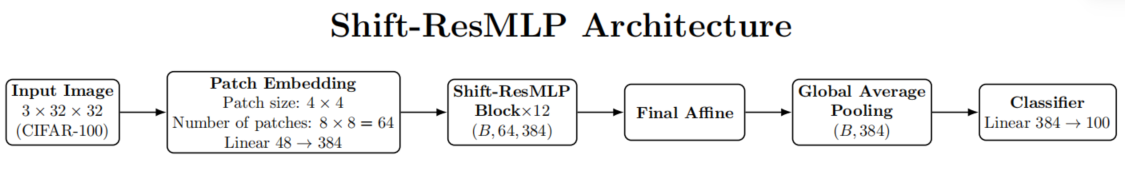
\includegraphics[width=0.98\textwidth]{figures/shift_resmlp_arch_official.png}
    \caption{Macro-architecture of Shift-ResMLP on CIFAR-100.}
    \label{fig:shift_resmlp_macro}
\end{subfigure}
\vspace{0.3em}
\begin{subfigure}[b]{\textwidth}
    \centering
    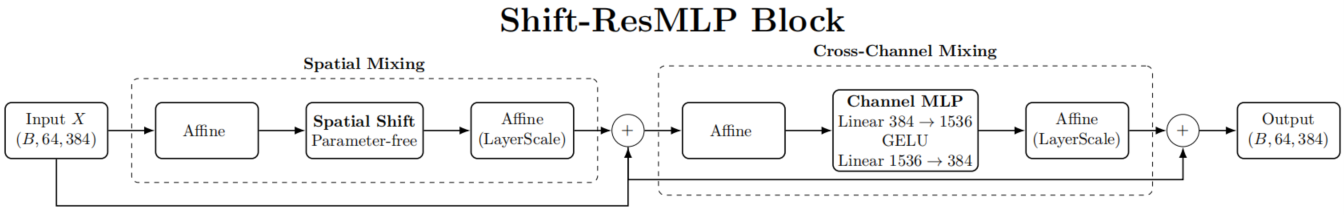
\includegraphics[width=0.98\textwidth]{figures/shift_resmlp_block.png}
    \caption{Shift-ResMLP block structure separating spatial mixing from cross-channel mixing.}
    \label{fig:shift_resmlp_block}
\end{subfigure}
\vspace{0.3em}
\begin{subfigure}[b]{0.63\textwidth}
    \centering
    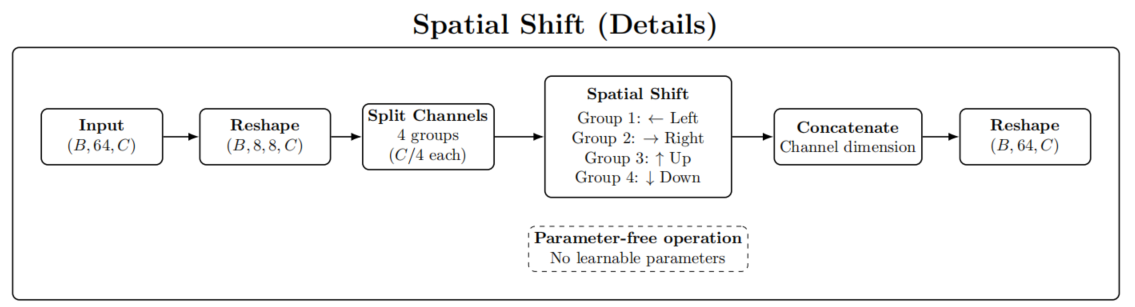
\includegraphics[width=\textwidth]{figures/spatial_shift_details.png}
    \caption{Parameter-free 4-direction coordinate shift mechanism.}
    \label{fig:spatial_shift_details}
\end{subfigure}
\hfill
\begin{subfigure}[b]{0.35\textwidth}
    \centering
    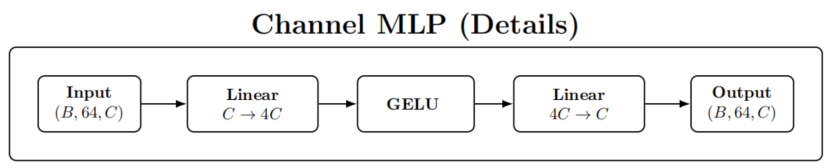
\includegraphics[width=\textwidth]{figures/channel_mlp_details.png}
    \caption{Channel MLP expansion.}
    \label{fig:channel_mlp_details}
\end{subfigure}
\vspace{0.3em}
\caption{Complete architectural design of Shift-ResMLP: macro dataflow, block-level residual paths, parameter-free 4-direction spatial communication, and channel feedforward projection.}
\label{fig:shift_resmlp_arch}
\end{figure}

\subsubsection{Components of Shift-ResMLP Block}
\label{subsubsection:shift_block}

A Shift-ResMLP block consists of two distinct sub-layers: a parameter-free spatial shift sub-layer and a cross-channel MLP sub-layer (Figure~\ref{fig:shift_resmlp_block}).

\textbf{Spatial mixing sub-layer} routes spatial information across tokens without matrix multiplication. Input tokens $\mathbf{x} \in \mathbb{R}^{B \times N \times C}$ are pre-normalized by an Affine layer and fed to the SpatialShift operator. The output is scaled by LayerScale parameter $\boldsymbol{\gamma}_1 \in \mathbb{R}^C$ and added back through a residual connection:
\begin{equation}
\mathbf{x} \leftarrow \mathbf{x} + \boldsymbol{\gamma}_1 \odot \text{SpatialShift}\big(\text{Affine}_1(\mathbf{x})\big).
\end{equation}

\textbf{Cross-channel mixing sub-layer} performs channel-wise feature transformation following spatial communication. Features pass through Affine normalization and a standard two-layer feedforward network: $\text{Linear}(C, 4C) \rightarrow \text{GELU} \rightarrow \text{Linear}(4C, C)$, scaled by LayerScale parameter $\boldsymbol{\gamma}_2$ and added to the residual path (Figure~\ref{fig:shift_resmlp_block}, \ref{fig:channel_mlp_details}):
\begin{equation}
\mathbf{x} \leftarrow \mathbf{x} + \boldsymbol{\gamma}_2 \odot \text{ChannelMLP}\big(\text{Affine}_2(\mathbf{x})\big).
\end{equation}

\subsubsection{Four-Direction Spatial Shift Mechanism}
\label{subsubsection:shift_mechanism}

\textbf{Coordinate feature partitioning} reshapes the 1D token sequence $\mathbf{x} \in \mathbb{R}^{B \times N \times C}$ into a 2D spatial feature map $\mathbf{X} \in \mathbb{R}^{B \times H \times W \times C}$, where $H = W = 32 / 4 = 8$ for patch size $P = 4$ on CIFAR-100. The channel dimension $C$ is partitioned into four equal, non-overlapping subsets of size $c = C / 4$ (Figure~\ref{fig:spatial_shift_details}):
\begin{enumerate}
    \item \textbf{Group 1 (Left Shift):} Channels $[0, c)$ are shifted left by 1 token and zero-padded on the right boundary:
      $\mathbf{X}'_{:, :, :-1, 0:c} = \mathbf{X}_{:, :, 1:, 0:c}$.
    \item \textbf{Group 2 (Right Shift):} Channels $[c, 2c)$ are shifted right by 1 token and zero-padded on the left boundary:
      $\mathbf{X}'_{:, :, 1:, c:2c} = \mathbf{X}_{:, :, :-1, c:2c}$.
    \item \textbf{Group 3 (Up Shift):} Channels $[2c, 3c)$ are shifted up by 1 token and zero-padded on the bottom boundary:
      $\mathbf{X}'_{:, :-1, :, 2c:3c} = \mathbf{X}_{:, 1:, :, 2c:3c}$.
    \item \textbf{Group 4 (Down Shift):} Channels $[3c, 4c)$ are shifted down by 1 token and zero-padded on the top boundary:
      $\mathbf{X}'_{:, 1:, :, 3c:4c} = \mathbf{X}_{:, :-1, :, 3c:4c}$.
\end{enumerate}

\textbf{Receptive field expansion} flattens the concatenated shifted tensor back to $(B, N, C)$. Because each block translates channels by 1 token in four orthogonal directions, stacking $L = 12$ blocks gradually broadens the effective receptive field across the entire $8*8$ grid, enabling global communication through repeated channel MLP mixing.

\subsubsection{Parameter Implications and Baseline Comparison}
\label{subsubsection:shift_params}

The SpatialShift operation contains \textbf{0 learnable parameters}. All model capacity resides in the linear patch embedding ($3 * 4^2 * C + C$) and the channel MLPs ($2 * C * 4C + 5C$ per block). For the experimental setting of $D = 384$ and $L = 12$ blocks:
\begin{equation}
P_{\text{Shift-ResMLP}} = 18,816 + 12 * 1,181,568 + 39,268 = \mathbf{14,264,548}.
\end{equation}
Compared to a standard columnar ResMLP of identical dimensions (ResMLPv2, with 14,314,468 parameters), Shift-ResMLP eliminates exactly $12 * (64 * 64 + 64) = 49,920$ spatial weights while preserving full 2D spatial connectivity.

\subsection{CA-Mixer: Resolution-Agnostic Cellular Automata}
\label{subsection:ca_mixer}

CA-Mixer addresses the resolution-locking bottleneck inherent in vision MLPs (Figure~\ref{fig:ca_mixer_arch}, \ref{fig:ca_scaling}). When image resolution increases from $32*32$ ($N=64$) to $64*64$ ($N=256$), a standard dense matrix $\mathbf{W} \in \mathbb{R}^{64 \times 64}$ fails due to dimensional mismatch. CA-Mixer resolves this by reformulating token mixing as an iterative Neural Cellular Automata (NCA) dynamical system~\cite{mordvintsev2020growing}. We describe its components below.

\begin{figure}[htbp]
\centering
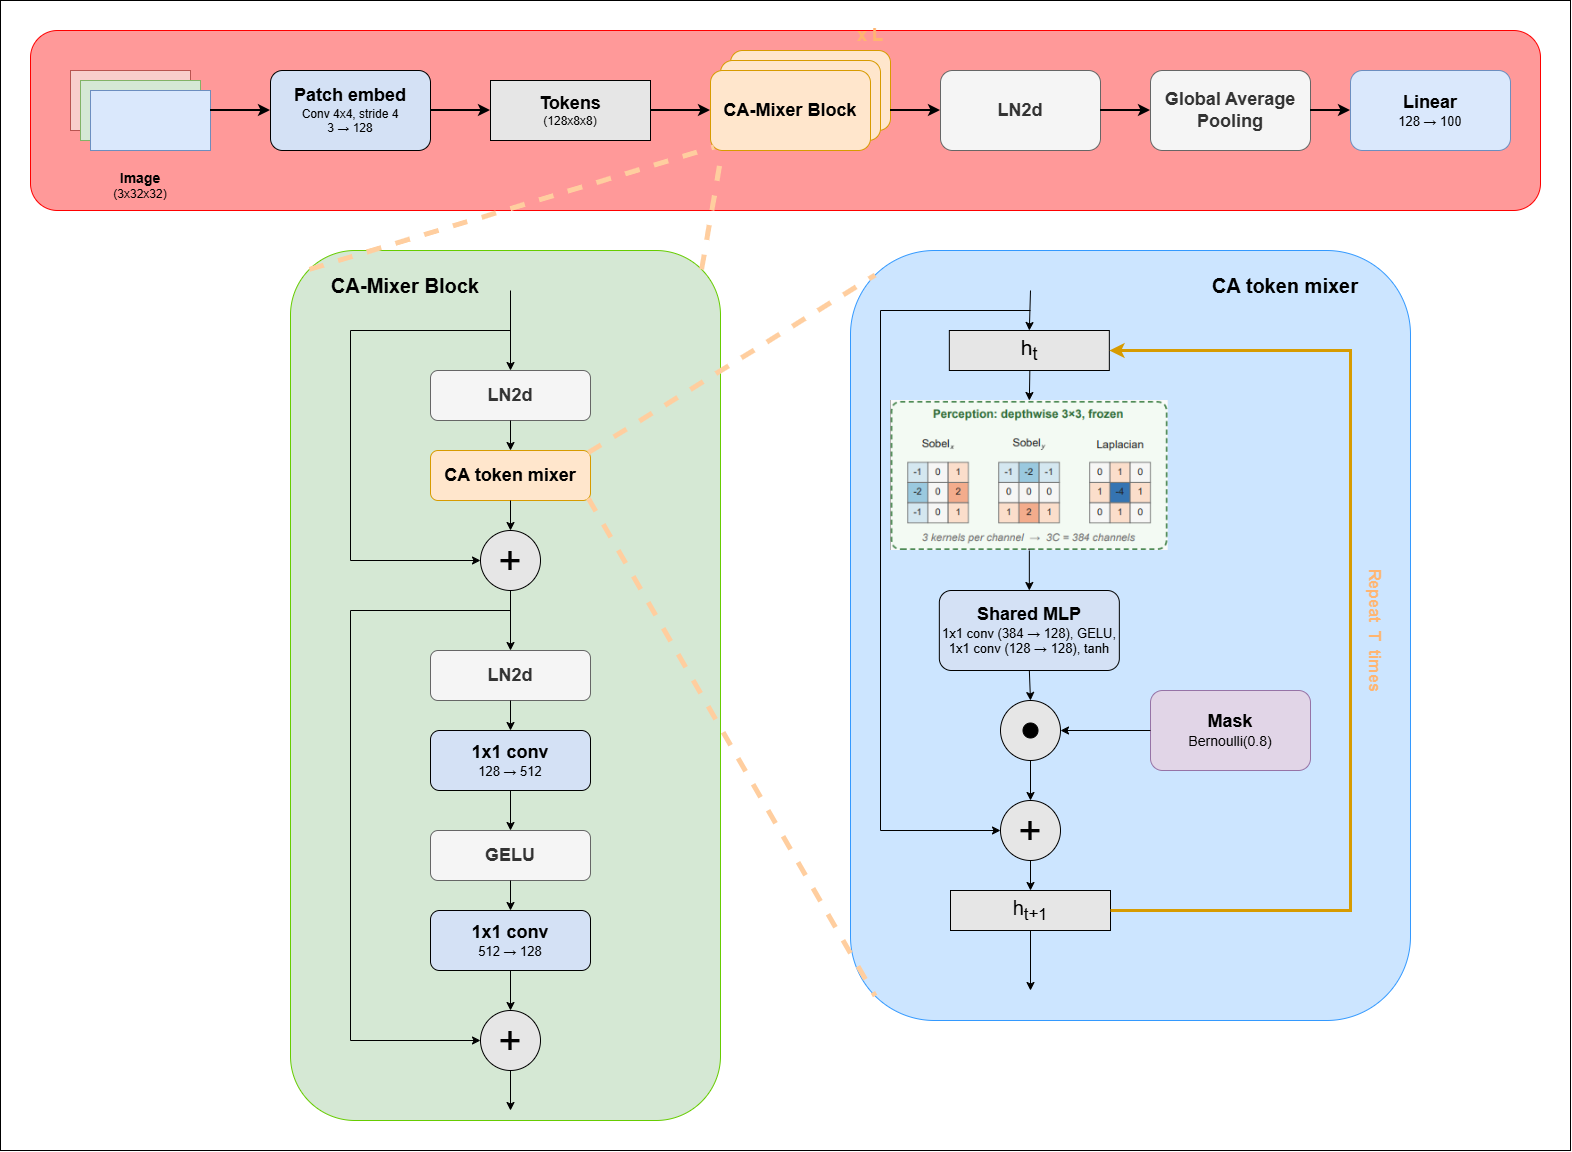
\includegraphics[width=0.92\textwidth]{figures/ca-mixer_model_architecture.png}
\caption{Macro-architecture and block design of CA-Mixer: patch embedding ($128 \times 8 \times 8$ tokens), CA-Mixer Block residual paths, and iterative Neural Cellular Automata (NCA) token mixer with frozen $3\times3$ depthwise Sobel/Laplacian perception kernels ($3C=384$), shared $1\times1$ conv MLP, and Bernoulli(0.8) stochastic update mask.}
\label{fig:ca_mixer_arch}
\end{figure}

\begin{figure}[htbp]
\centering
\begin{subfigure}[b]{0.92\textwidth}
    \centering
    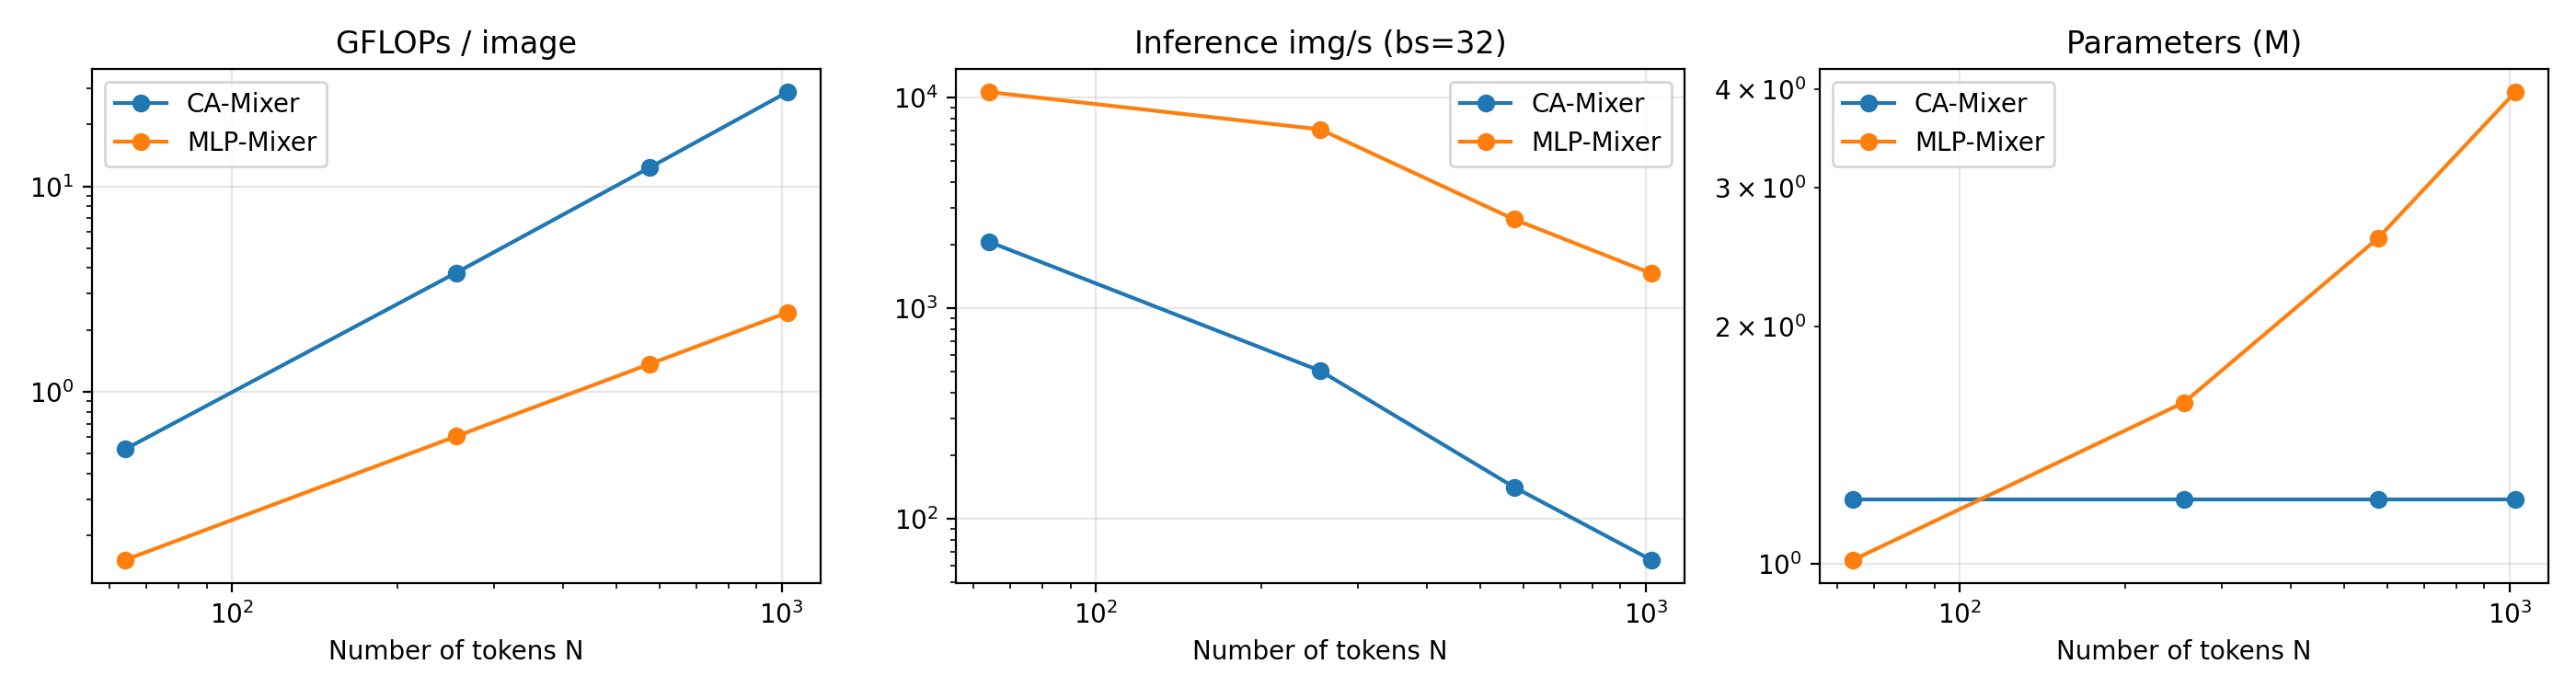
\includegraphics[width=\textwidth]{figures/fig_complexity.png}
    \caption{Parameter and FLOPs scaling vs. resolution.}
    \label{fig:ca_complexity}
\end{subfigure}
\vspace{0.5em}
\begin{subfigure}[b]{0.65\textwidth}
    \centering
    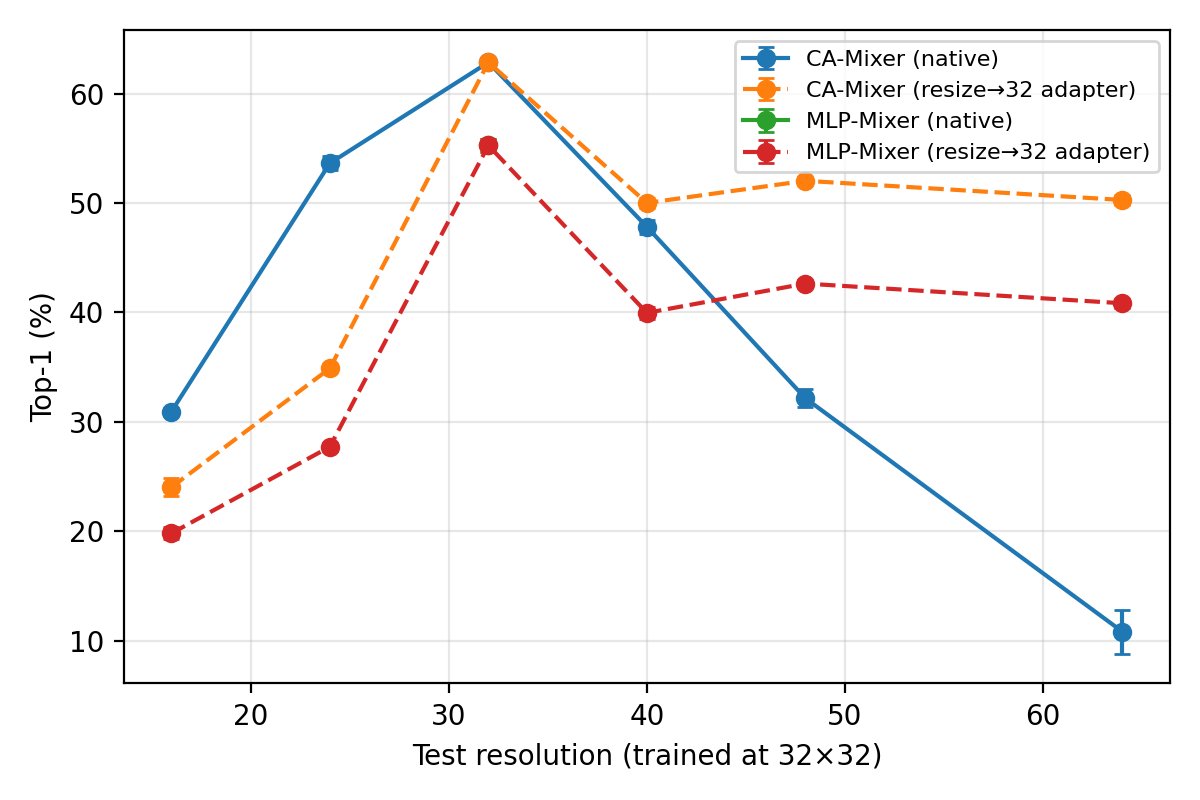
\includegraphics[width=\textwidth]{figures/fig_resolution.png}
    \caption{Zero-shot accuracy across resolutions.}
    \label{fig:ca_resolution}
\end{subfigure}
\vspace{0.3em}
\caption{Resolution invariance characteristics of CA-Mixer: constant parameter scaling and robust zero-shot accuracy under native resolution variations.}
\label{fig:ca_scaling}
\end{figure}

\textbf{Local differential perception operator} convolves the hidden state $\mathbf{h} \in \mathbb{R}^{B \times C \times H \times W}$ channel-wise with fixed, non-trainable spatial kernels $\mathbf{K} = [\text{Sobel}_X, \text{Sobel}_Y, \text{Laplacian}] \in \mathbb{R}^{3 \times 1 \times 3 \times 3}$. These biologically inspired filters capture directional spatial gradients and curvature without requiring learnable parameters.

\textbf{Shared update MLP} computes cell state increments $\mathbf{d}$ using shared $1*1$ convolutions across all spatial positions:
\begin{equation}
\mathbf{d} = \tanh\Big(\text{Conv}_{hidden \rightarrow C}\big(\text{GELU}(\text{Conv}_{3C \rightarrow hidden}(\mathbf{p}))\big)\Big),
\end{equation}
where $\mathbf{p}$ is the concatenated perception representation of dimension $3C$.

\textbf{Stochastic firing mask} introduces asynchronous update dynamics by sampling a binary mask $\mathbf{m} \sim \text{Bernoulli}(p = 0.8)$ during training. This prevents cells from over-relying on synchronous coordination and acts as strong spatial regularization.

\textbf{Iterative communication loop} repeats the state updates for $T = \max(H, W)$ recurrence steps:
\begin{equation}
\mathbf{h}_{t+1} = \mathbf{h}_t + \mathbf{m} \odot \mathbf{d}_t.
\end{equation}

\textbf{Resolution invariance property} ensures that because all perception and update operators are local 2D convolutions, the parameter count is completely decoupled from the spatial resolution $H \times W$. The compact model maintains exactly 1.21M parameters (1,207,524) while the scaled parameter-matched model maintains exactly 1.90M parameters (1,901,100) whether evaluated on $32*32$, $64*64$, or $128*128$ (Figure~\ref{fig:ca_scaling}).

\subsection{MetaFormer and Hybrid Paradigms: PoolFormer-S12 and HybridFormer}
\label{subsection:poolformer_hybridformer}

To contextualize our MLP models within the broader MetaFormer framework~\cite{yu2022metaformer}, we also analyze two hierarchical architectures: PoolFormer-S12 (Figure~\ref{fig:poolformer_arch}) and HybridFormer (Figure~\ref{fig:hybridformer_arch}).

\begin{figure}[htbp]
\centering
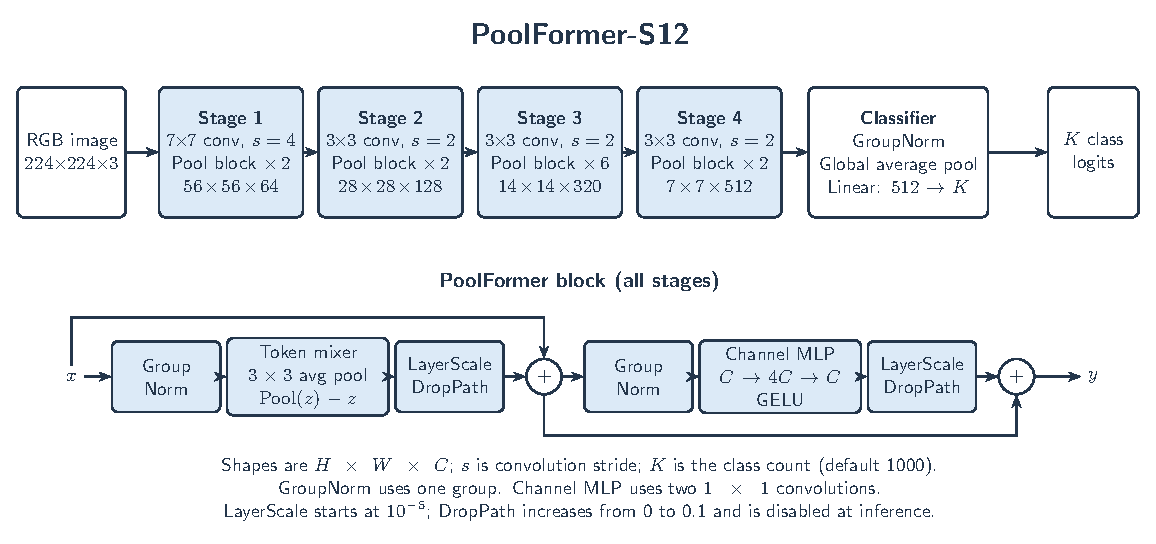
\includegraphics[width=0.98\textwidth]{figures/poolformer_arch.pdf}
\caption{Macro-architecture and block design of PoolFormer-S12: 4-stage hierarchical downsampling using non-parametric $3\times3$ average pooling for spatial token mixing.}
\label{fig:poolformer_arch}
\end{figure}

\begin{figure}[htbp]
\centering
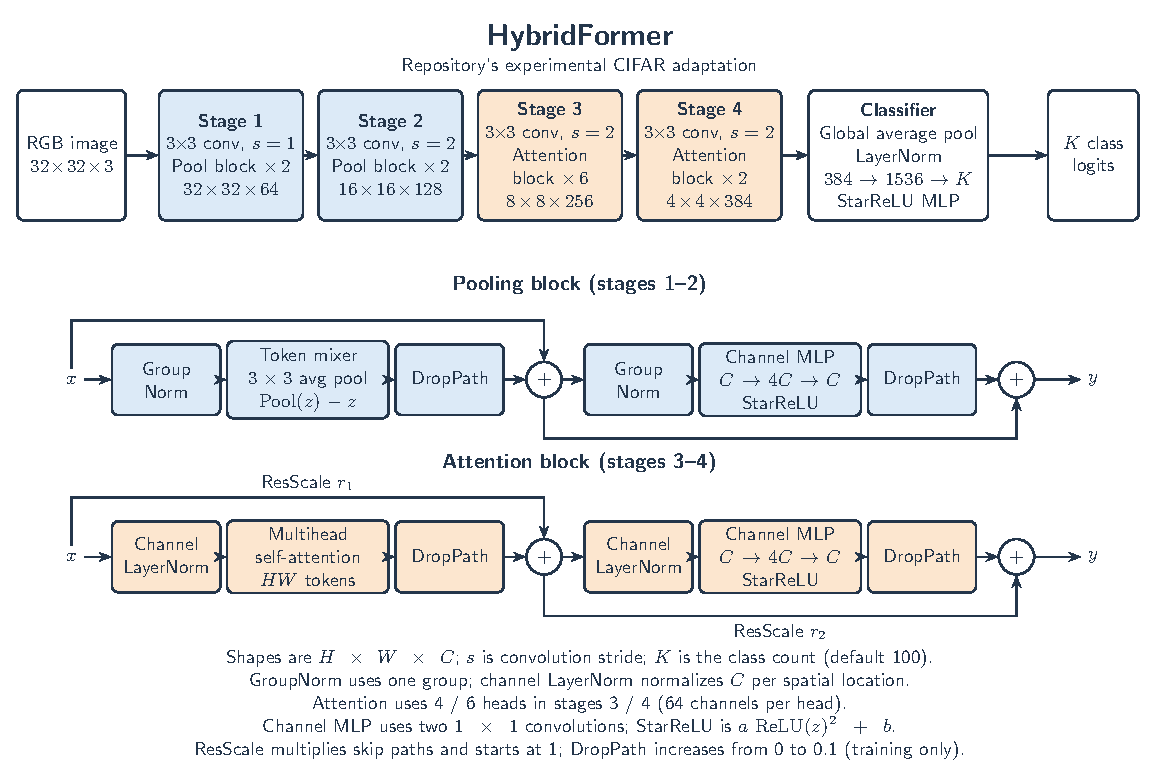
\includegraphics[width=0.98\textwidth]{figures/hybridformer_arch.pdf}
\caption{Macro-architecture of HybridFormer on CIFAR-100: combining parameter-free pooling blocks in Stages 1--2 with Multi-Head Self-Attention blocks in Stages 3--4 alongside StarReLU channel MLPs.}
\label{fig:hybridformer_arch}
\end{figure}

\subsubsection{PoolFormer-S12 Architecture}
\label{subsubsection:poolformer}

PoolFormer-S12 verifies the foundational premise of MetaFormer: that the macro-architecture itself, rather than specific token mixer parameters, delivers strong visual representations~\cite{yu2022metaformer}.

\textbf{Four-stage hierarchical downsampling} organizes the network into four stages with depths $[2, 2, 6, 2]$ and channel dimensions $[64, 128, 320, 512]$ (Figure~\ref{fig:poolformer_arch}). On $224*224$ inputs, a $7*7$ patch convolution stem with stride 4 reduces spatial resolution to $56*56$, followed by $3*3$ stride-2 convolutional downsamplers between subsequent stages.

\textbf{Non-parametric average pooling token mixer} replaces self-attention with a parameter-free spatial pooling operation:
\begin{equation}
\text{TokenMix}(\mathbf{x}) = \text{AvgPool2d}(\mathbf{x}, k=3, s=1, p=1) - \mathbf{x}.
\end{equation}
Subtracting the input tensor computes a residual difference representation without introducing a single learnable spatial weight.

\textbf{Channel MLP and normalization} refine features via two $1*1$ convolutions with expansion ratio 4 and GELU non-linearity, combined with GroupNorm (1 group, equivalent to LayerNorm over channels) and LayerScale initialized to $10^{-5}$. The complete architecture contains 11,453,476 parameters.

\subsubsection{HybridFormer Architecture}
\label{subsubsection:hybridformer}

HybridFormer combines parameter-free pooling with Multi-Head Self-Attention (MHSA) across hierarchical stages (Figure~\ref{fig:hybridformer_arch}).

\textbf{Multi-stage hybrid token mixing} assigns distinct mixing mechanisms to different resolution regimes: lightweight parameter-free pooling blocks in high-resolution early stages (Stages 1 and 2, at $32*32$ and $16*16$), and Multi-Head Self-Attention in low-resolution late stages (Stages 3 and 4, at $8*8$ and $4*4$). This avoids the quadratic complexity of self-attention on large token grids while preserving long-range relational reasoning in deep semantic stages.

\textbf{Multi-head self-attention with ResScale} in Stages 3 and 4 processes $HW$ tokens using 4 heads (Stage 3) and 6 heads (Stage 4) with head dimension 64, paired with channel LayerNorm and learnable skip scaling ($r_1, r_2$).

\textbf{StarReLU channel MLP} equips the feedforward network with StarReLU activation:
\begin{equation}
\text{StarReLU}(x) = s * (\text{ReLU}(x))^2 + b,
\end{equation}
where $s$ and $b$ are learnable scale and bias parameters. On native $32*32$ CIFAR-100 images, HybridFormer comprises 10,594,622 parameters.


\section{Experimental Setup and Training Protocols}
\label{section:experimental_setup}

This section outlines the benchmark datasets, training protocols, regularization strategies, and execution environments utilized across our Week 03 evaluations. Following standard practices established in modern vision Transformer and MLP literatures~\cite{ding2022repmlp, yu2022metaformer, touvron2021resmlp}, all models are evaluated under carefully controlled optimization recipes. We describe the datasets and evaluation metrics in Section~\ref{subsection:datasets}, detail the core training recipes and regularization schemes in Section~\ref{subsection:recipes}, present model-specific implementation settings in Section~\ref{subsection:member_pipelines}, and summarize all configurations in Table~\ref{tab:hyperparameters}.

\subsection{Datasets and Evaluation Metrics}
\label{subsection:datasets}

\textbf{CIFAR-100 dataset} consists of 60,000 $32*32$ color images divided across 100 fine-grained semantic categories (600 images per class). We partition the official 50,000 training images into 45,000 training samples and 5,000 validation samples using fixed random seed 42 to ensure deterministic reproducibility across all experimental runs, while reserving the remaining 10,000 images as the held-out test split.

\textbf{Tiny-ImageNet dataset} is employed to evaluate the scalability of our hierarchical models to higher image resolutions and larger class diversity. It comprises 100,000 training images and 10,000 validation images spanning 200 distinct ImageNet categories at $64*64$ resolution (500 training images per class).

\textbf{Evaluation metrics and calibration} are measured across several quantitative dimensions: Top-1 validation accuracy (\%), Top-5 validation accuracy (\%), cross-entropy loss, wall-clock training duration, and Expected Calibration Error (ECE). For models evaluated across multiple random seeds (such as CA-Mixer), we report the empirical mean alongside sample standard deviations ($\mu \pm \sigma$).

\subsection{Training Recipes and Optimization Protocols}
\label{subsection:recipes}

\textbf{Optimization and learning rate scheduling:} Following the training recipe of Touvron et al.~\cite{touvron2021resmlp} and Ding et al.~\cite{ding2022repmlp}, all models are trained using the AdamW optimizer~\cite{loshchilov2017adamw} with decoupled weight decay $\lambda = 0.05$. The learning rate follows a Cosine Annealing schedule~\cite{loshchilov2016sgdr} initialized at $\eta = 10^{-3}$ (or scaled according to batch size) and decayed gradually to a minimum threshold $\eta_{\text{min}} = 10^{-6}$ across epochs. Gradient clipping with a maximum norm of $1.0$ is enforced to prevent gradient instability during early optimization phases.

\textbf{Data augmentation suite:} To counteract overfitting and force models to learn robust invariant representations on compact datasets without ImageNet pretraining, we apply an intensive data augmentation pipeline. This includes RandAugment~\cite{cubuk2020randaugment} ($N=2, M=9$), Random Erasing~\cite{zhong2020random} ($p=0.1$ or $p=0.25$), Color Jitter ($0.1$), Mixup~\cite{zhang2017mixup} ($\alpha=0.8$), and CutMix~\cite{yun2019cutmix} ($\alpha=1.0$). Cross-entropy loss is computed with label smoothing $\epsilon = 0.1$.

\textbf{Stochastic depth (DropPath):} For deeper models and higher-resolution tasks where capacity can exceed the data manifold, stochastic depth~\cite{huang2016deep} is incorporated into residual paths. DropPath rate is set to $0.05$ on Tiny-ImageNet for Pyramid-ResMLP and $0.10$ for 4-stage MetaFormer models, linearly increasing across blocks from 0 to the target rate.

\textbf{Mixed precision and hardware acceleration:} All experiments utilize Automatic Mixed Precision (AMP FP16) to accelerate tensor operations and reduce GPU memory consumption without sacrificing numerical stability. Training is distributed across multi-GPU workstations and Kaggle accelerators using PyTorch Distributed Data Parallel (DDP).

\subsection{Model-Specific Experimental Pipelines}
\label{subsection:member_pipelines}

Because our team explored multiple architectural paradigms in parallel, individual experiments were executed under tailored training pipelines:

\textbf{Pyramid-ResMLP and Pyramid-ResMLP Pure} were benchmarked on our local multi-GPU workstation using distributed data parallel (DDP, 2 GPUs) via \texttt{src/engine/trainer.py}. Both models were trained for 100 epochs with batch size 256 using seed 42, AdamW optimizer, cosine learning rate decay ($\eta = 10^{-3} \rightarrow 10^{-6}$), and the complete vision augmentation suite (RandAugment, Random Erasing, Mixup, CutMix, label smoothing). On Tiny-ImageNet ($64*64$), batch size was set to 128 with initial learning rate $4*10^{-4}$ and weight decay $0.10$.

\textbf{Shift-ResMLP} was executed on a dedicated single-GPU CUDA environment using our standardized training engine. To comfortably fit the 12-block columnar architecture ($D=384$) in device memory, the per-device batch size was set to 128 over 100 epochs, utilizing identical AdamW optimization, Cosine schedule ($\eta = 10^{-3} \rightarrow 10^{-6}$), and vision augmentations.

\textbf{CA-Mixer} was implemented in \texttt{src/notebooks/ca\_mixer\_vs\_mlp\_mixer.ipynb} and evaluated on an NVIDIA Tesla T4 GPU. In addition to initial 30-epoch rapid exploratory runs ($1.21$M parameters, 3 seeds), CA-Mixer was systematically scaled to a parameter-matched configuration containing \textbf{1.90M parameters} ($C=160, D=6, C_{\text{nca}}=160, C_{\text{channel}}=652$) and trained for \textbf{100 epochs} (5 linear warmup epochs) with batch size 256, AdamW optimizer ($\eta = 10^{-3}$, $\lambda=0.05$), label smoothing $\epsilon=0.1$, step-budget ratio $\kappa=0.5$ ($T = \lceil 0.5 \times \max(H, W) \rceil = 4$ steps at $32\times32$), $T$-jitter of $0.25$, and update probability $0.8$ under AMP FP16. In-memory GPU tensor execution eliminated CPU data transfer overhead, maintaining a throughput of 3,942 images/second (35.0 seconds/epoch, 58.4 minutes total).

\textbf{PoolFormer-S12} was executed on Kaggle using 2x NVIDIA T4 GPUs under PyTorch Distributed Data Parallel (DDP). To maintain fidelity with the original MetaFormer paper~\cite{yu2022metaformer}, CIFAR-100 images were resized to $224*224$ via bicubic interpolation. Training ran for 100 epochs (5 warmup epochs) with a global batch size of 64 and a base learning rate scaled to $6.25*10^{-5}$ following the linear scaling rule ($10^{-3} \times 64 / 1024$). Vision augmentations followed the AutoAugment CIFAR-10 policy with Random Erasing ($0.25$), Mixup ($\alpha=0.8$), and CutMix ($\alpha=1.0$).

\textbf{HybridFormer} was executed on Kaggle using 2x NVIDIA T4 GPUs under DDP at native $32*32$ resolution. Due to the integration of multi-head self-attention in Stages 3 and 4, the model was trained for an extended schedule of 300 epochs (5 warmup epochs) with batch size 256, initial learning rate $5*10^{-4}$, and DropPath $0.10$.

\textbf{Hyperparameter summary across paradigms:} To enable a direct and systematic side-by-side comparison across these diverse training setups, all architectural hyperparameters, optimization schedules, vision augmentation configurations, and hardware allocations are compiled in Table~\ref{tab:hyperparameters}.

\begin{table}[htbp]
\centering
\begin{subtable}{\textwidth}
\centering
\footnotesize
\begin{tabularx}{\textwidth}{l | >{\centering\arraybackslash}X | >{\centering\arraybackslash}X | >{\centering\arraybackslash}X | >{\centering\arraybackslash}X}
\toprule
\textbf{Hyperparameter} & \textbf{Pyramid-ResMLP Pure} & \textbf{Pyramid-ResMLP} & \textbf{Shift-ResMLP} & \textbf{CA-Mixer} \\
\midrule
Target Dataset & CIFAR-100 & CIFAR-100 & CIFAR-100 & CIFAR-100 \\
Input Resolution & $32 \times 32$ & $32 \times 32$ & $32 \times 32$ & $32 \times 32$ \\
Total Epochs & 100 & 100 & 100 & 100 \\
Batch Size & 256 & 256 & 128 & 256 \\
Optimizer & AdamW & AdamW & AdamW & AdamW \\
Initial Learning Rate ($\eta$) & $10^{-3}$ & $10^{-3}$ & $10^{-3}$ & $10^{-3}$ \\
LR Schedule & Cosine (to $10^{-6}$) & Cosine (to $10^{-6}$) & Cosine (to $10^{-6}$) & Cosine (to $10^{-6}$) \\
Warmup Epochs & 0 & 0 & 0 & 5 \\
Weight Decay ($\lambda$) & 0.05 & 0.05 & 0.05 & 0.05 \\
Gradient Clipping & Norm 1.0 & Norm 1.0 & Norm 1.0 & Norm 1.0 \\
Data Augmentation & RandAugment, Erasing, Jitter & RandAugment, Erasing, Jitter & RandAugment, Erasing, Jitter & GPU Crop, HFlip \\
Mixup / CutMix ($\alpha_1, \alpha_2$) & 0.8 / 1.0 & 0.8 / 1.0 & 0.8 / 1.0 & None \\
Label Smoothing ($\epsilon$) & 0.1 & 0.1 & 0.1 & 0.1 \\
DropPath Rate & None & None & None & None \\
Compute Hardware & 2$\times$ GPUs (DDP) & 2$\times$ GPUs (DDP) & 1$\times$ CUDA GPU & 1$\times$ Tesla T4 (in-memory) \\
Mixed Precision & AMP FP16 & AMP FP16 & AMP FP16 & AMP FP16 \\
\bottomrule
\end{tabularx}
\vspace{0.3em}
\caption{Primary Vision MLP candidates on CIFAR-100 (CA-Mixer listed at 100-epoch scaled configuration; initial exploration evaluated at 30 epochs with 2 warmup epochs).}
\label{tab:hyperparams_mlps}
\end{subtable}

\vspace{0.6em}

\begin{subtable}{\textwidth}
\centering
\footnotesize
\begin{tabularx}{\textwidth}{l | >{\centering\arraybackslash}X | >{\centering\arraybackslash}X | >{\centering\arraybackslash}X}
\toprule
\textbf{Hyperparameter} & \textbf{PoolFormer-S12} & \textbf{HybridFormer} & \textbf{Pyramid-ResMLP (Scaled)} \\
\midrule
Target Dataset & CIFAR-100 & CIFAR-100 & Tiny-ImageNet (200 Classes) \\
Input Resolution & $224 \times 224$ (bicubic) & $32 \times 32$ (native) & $64 \times 64$ (native) \\
Total Epochs & 100 & 300 & 100 \\
Batch Size & 64 ($32 \times 2$) & 256 ($128 \times 2$) & 128 (DDP) \\
Optimizer & AdamW & AdamW & AdamW \\
Initial Learning Rate ($\eta$) & $6.25 \times 10^{-5}$ & $5 \times 10^{-4}$ & $4 \times 10^{-4}$ \\
LR Schedule & Cosine (to $10^{-6}$) & Cosine (to $10^{-6}$) & Cosine (to $10^{-6}$) \\
Warmup Epochs & 5 & 5 & 0 \\
Weight Decay ($\lambda$) & 0.05 & 0.05 & 0.10 \\
Gradient Clipping & None & Norm 1.0 & Norm 1.0 \\
DropPath Rate & 0.10 & 0.10 & 0.05 \\
Data Augmentation & AutoAugment, Erasing & AutoAugment, Erasing & RandAugment, Erasing (0.25) \\
Mixup / CutMix ($\alpha_1, \alpha_2$) & 0.8 / 1.0 & 0.8 / 1.0 & 0.8 / 1.0 \\
Label Smoothing ($\epsilon$) & 0.1 & 0.1 & 0.1 \\
Compute Hardware & 2$\times$ Kaggle T4 (DDP) & 2$\times$ Kaggle T4 (DDP) & 2$\times$ GPUs (DDP) \\
Mixed Precision & AMP FP16 & AMP FP16 & AMP FP16 \\
\bottomrule
\end{tabularx}
\vspace{0.3em}
\caption{MetaFormer baselines and scaled high-resolution benchmark.}
\label{tab:hyperparams_baselines}
\end{subtable}
\vspace{0.4em}
\caption{Comprehensive hyperparameter and training setup comparison across all models investigated in Week 03, partitioned into (a) primary Vision MLP candidates on CIFAR-100 and (b) MetaFormer baselines and scaled high-resolution benchmarks.}
\label{tab:hyperparameters}
\end{table}
\clearpage


\section{Empirical Results and Comparative Analysis}
\label{section:results}

\subsection{Master Benchmark Results}
Table~\ref{tab:benchmark_master} compiles the primary empirical results across all architectures evaluated on CIFAR-100 alongside the Week 02 baselines.

\begin{table}[htbp]
\centering
\begin{adjustbox}{max width=\textwidth}
\small
\setlength{\tabcolsep}{5pt}
\begin{tabular}{lllrcrr}
\toprule
\textbf{Model Architecture} & \textbf{Paradigm} & \textbf{Spatial Token Mixer} & \textbf{Params} & \textbf{Epochs} & \textbf{Top-1 Val (\%)} & \textbf{Train Time} \\
\midrule
ResMLP Baseline & Isotropic & Pure Linear $(N \times N)$ & 2.19M & 100 & 62.40\% & 54.6 min \\
RepMLP Baseline & Hierarchical & RepConv 3-Branch & 2.16M & 100 & 71.46\% & 107.1 min \\
\textbf{Pyramid-ResMLP Pure} & Hierarchical & Linear $(N_i \times N_i)$ & \textbf{1.93M} & 100 & \textbf{68.22\%} & \textbf{44.9 min} \\
\textbf{Pyramid-ResMLP} & Hierarchical & RepToken (Fused)$^*$ & \textbf{1.79M} & 100 & \textbf{72.18\%} & \textbf{44.5 min} \\
\textbf{Shift-ResMLP} & Isotropic & 4-Direction Shift & 14.26M & 100 & \textbf{72.92\%} & 110.2 min \\
\textbf{CA-Mixer} & Isotropic NCA & Cellular Automata & \textbf{1.90M} & 100 & \textbf{64.92\%} & \textbf{58.4 min} \\
PoolFormer-S12 & Hierarchical & Non-parametric AvgPool$^\dagger$ & 11.45M & 100 & 59.50\% & $\sim$53 min \\
HybridFormer & Hierarchical & PoolFormer + MHSA & 10.59M & 300 & \textbf{75.70\%} & $\sim$160 min \\
\bottomrule
\end{tabular}
\end{adjustbox}
\vspace{0.4em}
\caption{Empirical performance benchmark on CIFAR-100 across architectural paradigms. $^*$Pyramid-ResMLP contains 1.94M training parameters (1,938,820) which structurally fuse into 1.79M (1,785,828) upon deployment. CA-Mixer scales to 64.92\% Top-1 validation accuracy at 1.90M parameters (1,901,100 params, 0.489 GFLOPs, 2.20\% ECE, 58.4 min) over 100 epochs, compared to 62.87\% in the 30-epoch 1.21M fast exploration (20.0 min). $^\dagger$PoolFormer-S12 is evaluated at $224 \times 224$ following the canonical MetaFormer training setup~\cite{yu2022metaformer}.}
\label{tab:benchmark_master}
\end{table}

\subsection{Training Dynamics and Learning Profiles}
Because experimental schedules varied across paradigms (100 epochs for our primary models, 30 epochs for rapid CA-Mixer exploration, and 300 epochs for HybridFormer), we analyze their learning trajectories based on their respective optimization dynamics and generalization behavior.

\begin{figure}[htbp]
\centering
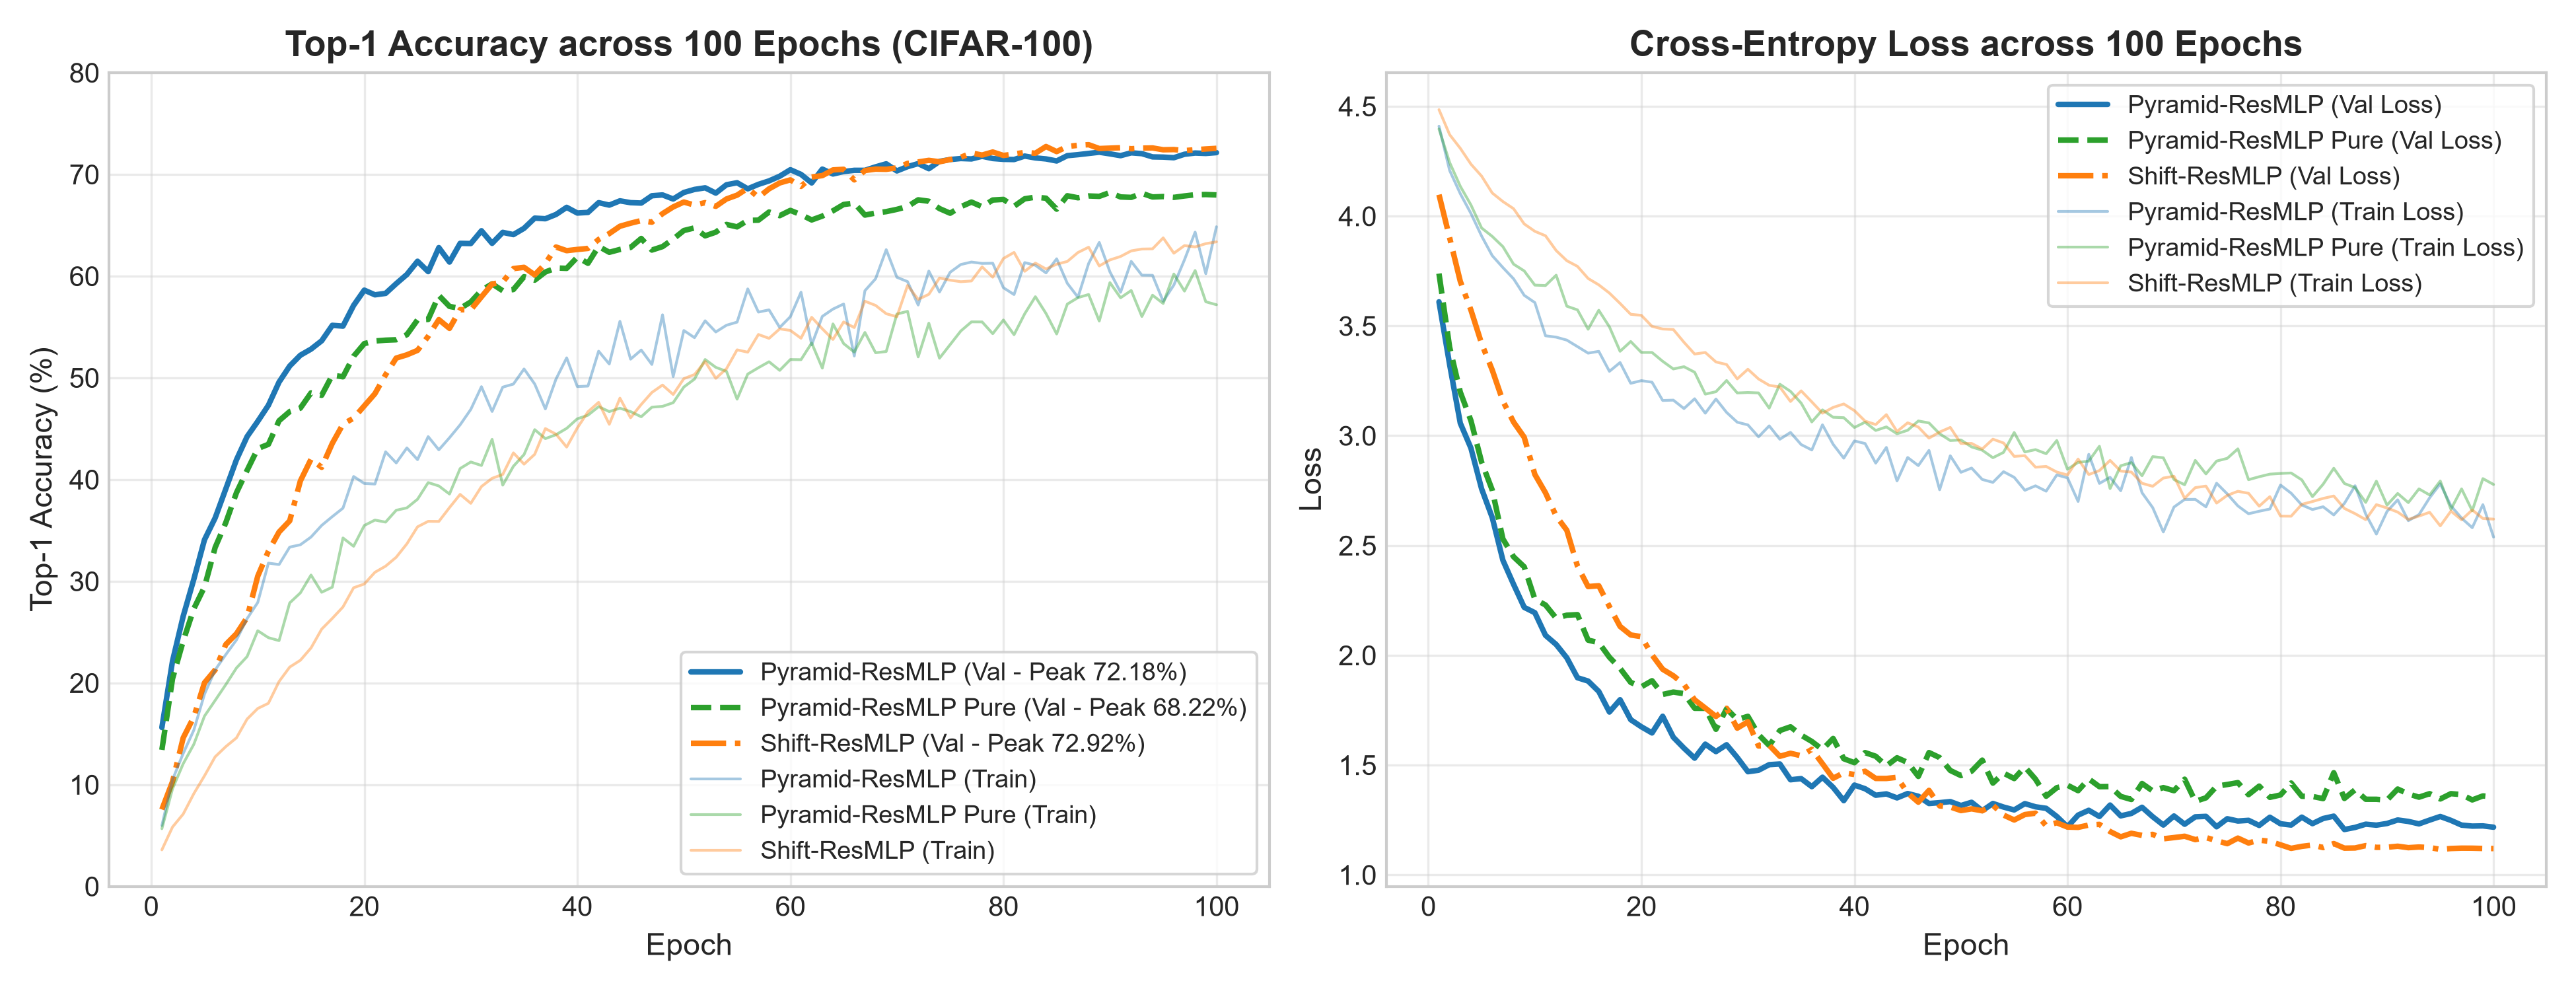
\includegraphics[width=\textwidth]{figures/training_curves_comparison.png}
\caption{Training and validation dynamics across 100 epochs on CIFAR-100 comparing Pyramid-ResMLP, Pyramid-ResMLP Pure, and Shift-ResMLP.}
\label{fig:curves_comparison}
\end{figure}

\subsubsection{Convergence Behavior of Pyramid Models and Shift-ResMLP}
Figure~\ref{fig:curves_comparison} compares the Top-1 validation accuracy and cross-entropy loss trajectories for our three 100-epoch CIFAR-100 runs. Table~\ref{tab:epoch_progress} provides numerical checkpoints partitioned into validation accuracy and cross-entropy loss trajectories.

\begin{table}[htbp]
\centering
\begin{subtable}{\textwidth}
\centering
\small
\begin{tabularx}{\textwidth}{c*{3}{>{\centering\arraybackslash}X}}
\toprule
\textbf{Epoch} & \textbf{Pyramid-ResMLP Pure} & \textbf{Pyramid-ResMLP} & \textbf{Shift-ResMLP} \\
\midrule
1  & 13.42\% & 15.62\% & 7.56\% \\
10 & 43.04\% & 45.72\% & 30.50\% \\
20 & 53.36\% & 58.62\% & 47.24\% \\
40 & 61.86\% & 66.20\% & 62.62\% \\
60 & 66.46\% & 70.46\% & 69.46\% \\
80 & 67.54\% & 71.48\% & 71.86\% \\
\midrule
\textbf{Peak} & \textbf{68.22\%} (Epoch 90) & \textbf{72.18\%} (Epoch 89) & \textbf{72.92\%} (Epoch 88) \\
100 & 67.98\% & 72.14\% & 72.56\% \\
\bottomrule
\end{tabularx}
\vspace{0.3em}
\caption{Top-1 Validation Accuracy Trajectory (\%).}
\label{tab:val_acc_trajectory}
\end{subtable}

\vspace{0.8em}

\begin{subtable}{\textwidth}
\centering
\small
\begin{tabularx}{\textwidth}{c*{3}{>{\centering\arraybackslash}X}}
\toprule
\textbf{Epoch} & \textbf{Pyramid-ResMLP Pure} & \textbf{Pyramid-ResMLP} & \textbf{Shift-ResMLP} \\
\midrule
1  & 3.7385 & 3.6098 & 4.0979 \\
10 & 2.2554 & 2.1938 & 2.8236 \\
20 & 1.8562 & 1.6741 & 2.0848 \\
40 & 1.5107 & 1.4088 & 1.4567 \\
60 & 1.4081 & 1.2189 & 1.2175 \\
80 & 1.3638 & 1.2324 & 1.1366 \\
\midrule
\textbf{Peak} & \textbf{1.3402} (Epoch 90) & \textbf{1.2262} (Epoch 89) & \textbf{1.1330} (Epoch 88) \\
100 & 1.3546 & 1.2169 & 1.1197 \\
\bottomrule
\end{tabularx}
\vspace{0.3em}
\caption{Validation Cross-Entropy Loss Trajectory.}
\label{tab:val_loss_trajectory}
\end{subtable}
\vspace{0.5em}
\caption{Validation convergence dynamics across 100 epochs on CIFAR-100, comparing (a) Top-1 validation accuracy (\%) and (b) validation cross-entropy loss trajectories between Pyramid-ResMLP Pure, Pyramid-ResMLP, and Shift-ResMLP.}
\label{tab:epoch_progress}
\end{table}

Key observations from the training curves include:
\begin{itemize}
    \item \textbf{Regularization inverted gap in early epochs:} In all three models, training accuracy appears lower than validation accuracy for the first 40 epochs. This is expected behavior caused by heavy data augmentations (Mixup with $\alpha=0.8$, CutMix with $\alpha=1.0$, and RandAugment), which corrupt training images to prevent early memorization, while validation evaluation runs on clean images.
    \item \textbf{Accelerated convergence of Pyramid-ResMLP:} Pyramid-ResMLP consistently outpaces Pyramid-ResMLP Pure by $3-5\%$ throughout the training run. By epoch 20, Pyramid-ResMLP achieves 58.62\% validation accuracy, whereas Pyramid-ResMLP Pure reaches 53.36\% and Shift-ResMLP reaches 47.24\%.
    \item \textbf{Late-epoch stabilization:} All three models reach their peak performance between epochs 88 and 90, corresponding to the final annealing phase of the Cosine learning rate schedule where the step size reaches $\eta_{\text{min}} = 10^{-6}$.
\end{itemize}

\subsubsection{Convergence Dynamics and 100-Epoch Scaling in CA-Mixer}
To rigorously evaluate whether Neural Cellular Automata token mixing scales with model capacity and extended training schedules, CA-Mixer was benchmarked under two distinct regimes:
\begin{itemize}
    \item \textbf{Compact 30-epoch rapid exploration (1.21M parameters):} Processing in-memory GPU tensors without data augmentation bottlenecks required only 20.0 minutes across three random seeds ($62.87 \pm 0.24\%$ Top-1 validation accuracy, $88.09 \pm 0.30\%$ Top-5). CA-Mixer constrained the train-test generalization gap to $20.74 \pm 0.56\%$ (slashing overfitting by over 17\% compared to unconstrained dense mixers) and attained an Expected Calibration Error (ECE) of $3.82 \pm 0.22\%$.
    \item \textbf{Parameter-matched 100-epoch scaling (1.90M parameters):} Scaling CA-Mixer to 1.90M parameters ($C=160, D=6, C_{\text{nca}}=160, C_{\text{channel}}=652$) directly matches the parameter budget of Pyramid-ResMLP Pure (1.93M) and Pyramid-ResMLP (1.94M train / 1.79M deploy). When trained for 100 epochs with AdamW ($\eta = 10^{-3}, \lambda = 0.05$) and dynamic step jitter ($T_{\text{jitter}}=0.25$, $T=4$ at $32\times32$, 0.489 GFLOPs/image), CA-Mixer achieves \textbf{64.92\%} Top-1 accuracy, \textbf{85.72\%} Top-5 accuracy, and a test loss of $1.503$ in 58.4 minutes (35.0 seconds/epoch, 3,942 images/second on a single Tesla T4 GPU, Figure~\ref{fig:ca_100ep_curves}). Furthermore, the Expected Calibration Error is reduced to an outstanding \textbf{2.20\%}, establishing CA-Mixer as the most well-calibrated architecture among all evaluated models.
\end{itemize}
These results demonstrate that the inductive bias provided by fixed differential spatial operators ($\text{Sobel}_X, \text{Sobel}_Y, \text{Laplacian}$) not only guarantees complete resolution invariance, but also provides strong spatial regularization and calibrated predictive uncertainty across extended training schedules.

\begin{figure}[htbp]
\centering
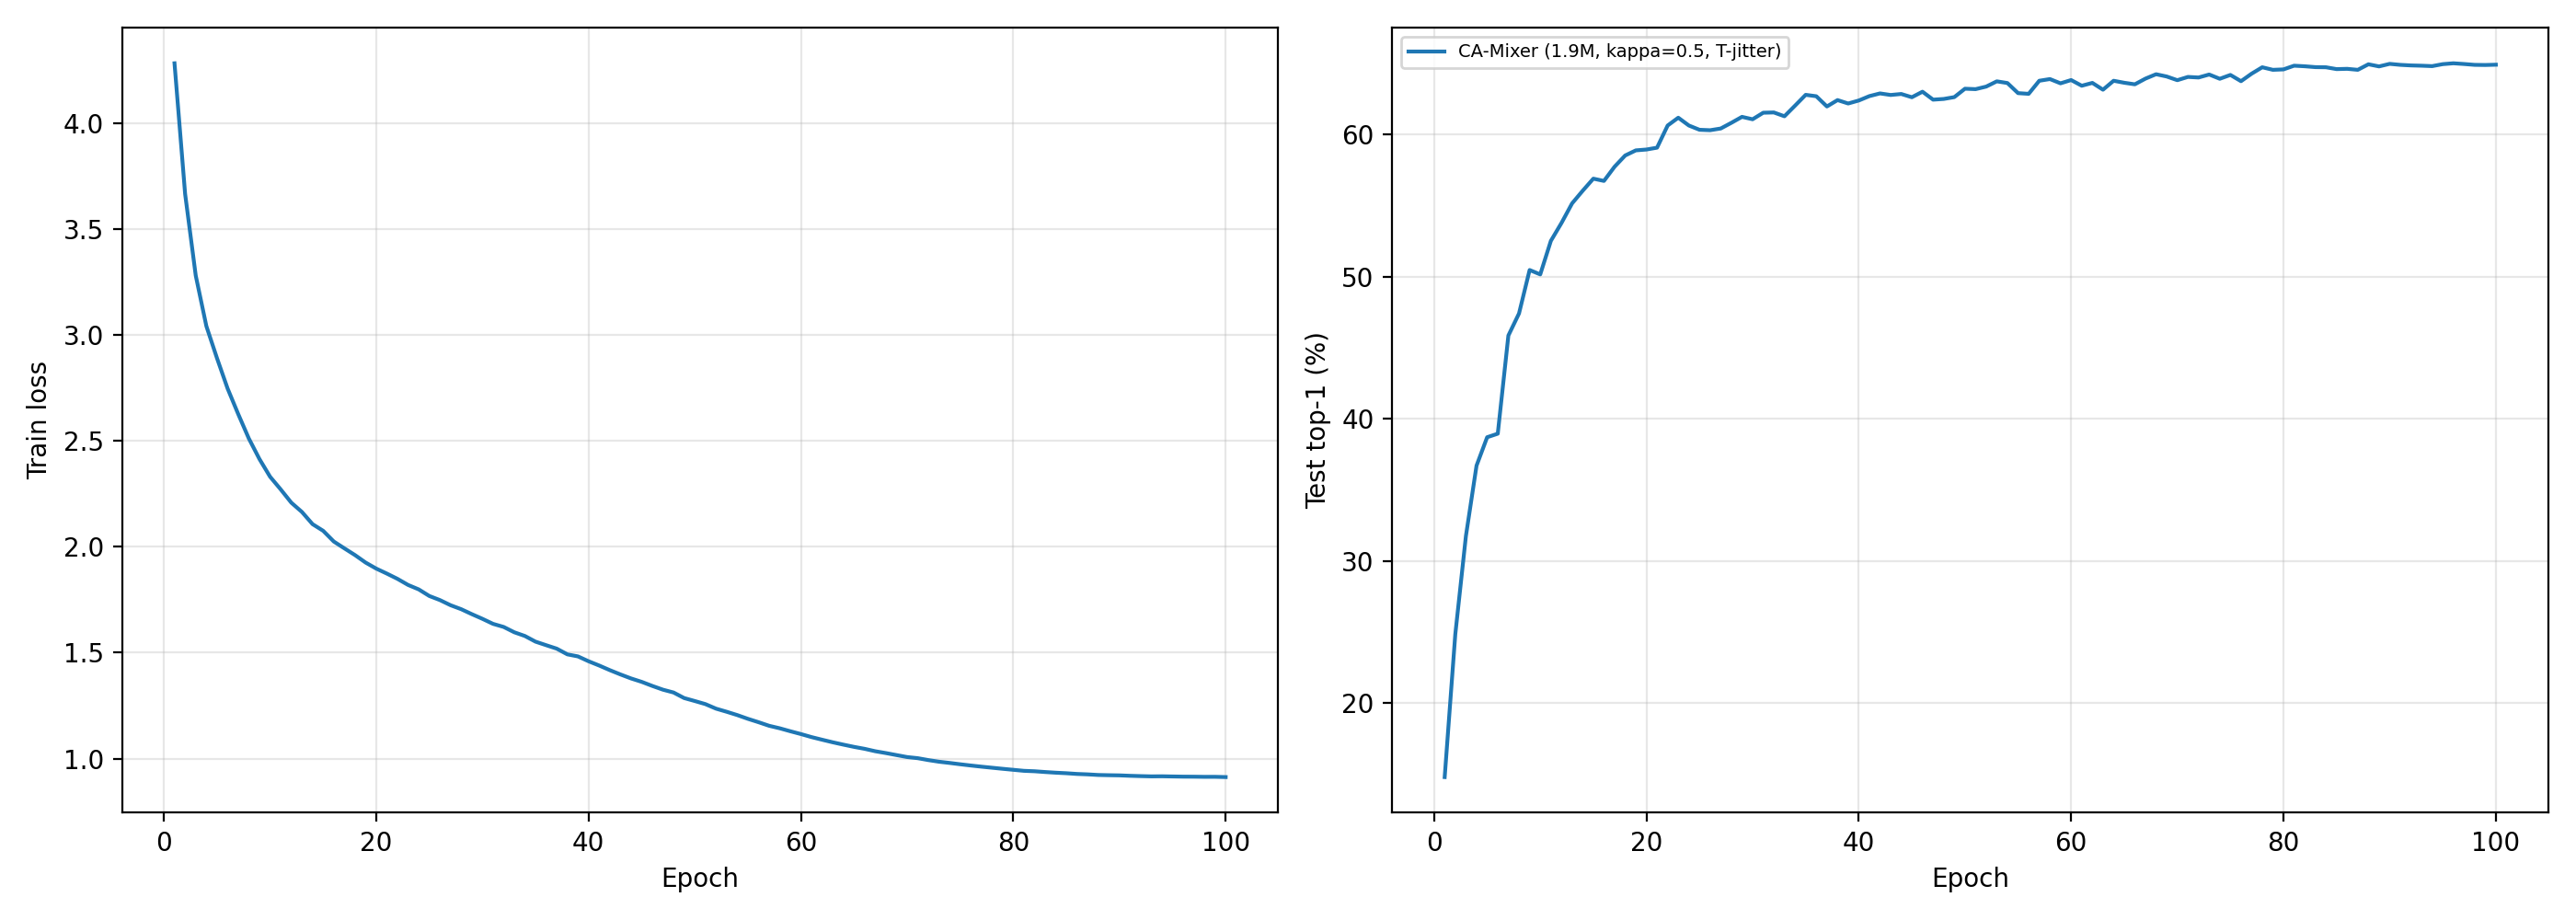
\includegraphics[width=0.98\textwidth]{figures/ca_100ep_training_curves.png}
\caption{Training loss (left) and test Top-1 validation accuracy (right) trajectories of CA-Mixer (1.90M parameters, $\kappa=0.5$, $T$-jitter) across 100 epochs on CIFAR-100.}
\label{fig:ca_100ep_curves}
\end{figure}

\subsubsection{Extended 300-Epoch Trajectory in HybridFormer}
In HybridFormer, the inclusion of multi-head self-attention in Stages 2 and 3 necessitates a longer optimization schedule. While the model reaches 65\% accuracy around epoch 100, continued training enables the attention layers to refine long-range semantic dependencies, ultimately peaking at \textbf{75.70\%} validation accuracy at epoch 275 and achieving \textbf{75.27\%} on the held-out test set.

\subsection{Scaling to Tiny-ImageNet (\texorpdfstring{$64 \times 64$}{64x64}, 200 Classes)}
To evaluate whether the pyramid architecture scales to higher spatial dimensions and larger class counts, we benchmarked Pyramid-ResMLP on Tiny-ImageNet across two distinct structural and regularization configurations, summarized in Table~\ref{tab:tiny_imagenet_scaling}:
\begin{itemize}
    \item \textbf{Base Configuration ($C=[96, 192, 384]$, $B=[2, 4, 6]$):} Containing 9.37M deployable parameters, the base model achieved 57.85\% Top-1 validation accuracy. However, signs of overfitting emerged as training accuracy reached 69.08\% while validation loss began to plateau around 2.0546.
    \item \textbf{Scaled Configuration with DropPath ($C=[112, 224, 448]$, $B=[2, 4, 6]$):} Increasing channel capacity to 12.73M deployable parameters while introducing stochastic depth ($\text{DropPath} = 0.05$), higher weight decay ($\lambda = 0.10$), and random erasing ($p=0.25$) improved Top-1 accuracy to \textbf{62.93\%} (and Top-5 accuracy to \textbf{82.83\%}). The $+5.08\%$ improvement confirms that stochastic depth effectively regularizes multi-stage pyramid MLPs on higher-resolution inputs.
\end{itemize}

\begin{table}[htbp]
\centering
\small
\begin{tabularx}{\textwidth}{l >{\raggedright\arraybackslash}X r r r}
\toprule
\textbf{Model Configuration} & \textbf{Channels, Depths, and Regularization} & \textbf{Deploy Params} & \textbf{Top-1 Val} & \textbf{Top-5 Val} \\
\midrule
Pyramid-ResMLP (Base) & $C=[96, 192, 384]$, $B=[2, 4, 6]$, $\lambda=0.05$ & 9,370,760 & 57.85\% & 79.12\% \\
\textbf{Pyramid-ResMLP (DropPath)} & $C=[112, 224, 448]$, $B=[2, 4, 6]$, DropPath 0.05, Erase 0.25 & \textbf{12,728,104} & \textbf{62.93\%} & \textbf{82.83\%} \\
\bottomrule
\end{tabularx}
\vspace{0.4em}
\caption{High-resolution scaling benchmark of Pyramid-ResMLP on Tiny-ImageNet ($64 \times 64$, 200 classes) across 100 epochs.}
\label{tab:tiny_imagenet_scaling}
\end{table}

\subsection{Hypothesis Verification: Resolving Parameter Inefficiency}
Our empirical findings definitively answer the research question formulated at the end of Week 02:

\subsubsection{The Two-Step Ablation Proof}
By comparing vanilla ResMLP, Pyramid-ResMLP Pure, and Pyramid-ResMLP, we isolate the exact source of performance gains:
\begin{align}
\text{ResMLP Isotropic (62.40\%)} &\xrightarrow{\mathbf{+5.82\%}} \text{Pyramid-ResMLP Pure (68.22\%)} \nonumber \\
&\xrightarrow{\mathbf{+3.96\%}} \text{Pyramid-ResMLP (72.18\%)}.
\end{align}
\begin{enumerate}
    \item \textbf{Step 1 (Hierarchical Pyramid):} Transitioning from a single-scale column to a 3-stage pyramid improves Top-1 accuracy by \textbf{+5.82\%} while saving 265k parameters and reducing training time from 54.65 to 44.91 minutes. This confirms that multi-scale downsampling provides crucial spatial abstraction.
    \item \textbf{Step 2 (Structural Re-parameterization):} Adding parallel depthwise convolutions during training contributes an additional \textbf{+3.96\%}. Because these branches fuse into the linear layer upon deployment, this gain incurs \textbf{zero inference latency or parameter overhead}.
\end{enumerate}

\subsubsection{Shift-ResMLP vs. Pyramid-ResMLP Tradeoff}
Shift-ResMLP demonstrates that spatial communication can achieve \textbf{72.92\%} accuracy with strictly zero learnable spatial weights. However, because Shift-ResMLP remains an isotropic columnar model, it requires 14.26M parameters and 110.21 minutes of training to achieve this score. In contrast, Pyramid-ResMLP reaches 72.18\% with only \textbf{1.79M deployable parameters} (an 8-fold reduction in parameter size) and trains in less than half the time (44.53 minutes), establishing hierarchical feature downsampling as the superior architectural paradigm.


\section{Challenges, Consultation with TA, and Week 04 Roadmap}
\label{section:roadmap}

\subsection{Technical Challenges Encountered in Week 03}
During our Week 03 exploration, our team identified several technical hurdles:
\begin{itemize}
    \item \textbf{a. Channel capacity inflation in single-stage models:} While Shift-ResMLP successfully achieved 72.92\% accuracy with parameter-free spatial mixing, its isotropic single-scale nature required a large channel width ($D = 384$) and 12 blocks, accumulating 14.26 million parameters. In contrast, multi-stage pyramids achieve comparable performance with 1.79 million parameters, confirming that isotropic backbones suffer from intrinsic capacity inefficiency.
    \item \textbf{b. Regularization requirements at higher resolutions:} On Tiny-ImageNet ($64*64$), our base pyramid model exhibited overfitting due to increased spatial token counts. Introducing stochastic depth (DropPath = 0.05) and heavier weight decay was essential to unlock strong generalization (+5.08\% improvement to 62.93\%), indicating that regularization becomes increasingly critical as resolution scales up.
    \item \textbf{c. Disparate peer training pipelines:} Because team members worked on diverse compute environments (local DDP clusters, single CUDA GPUs, and Kaggle T4 accelerators), differing batch sizes, learning rates, and augmentation suites made cross-model comparison nuanced. A primary goal for Week 04 is unifying all top-performing candidates under an identical benchmarking harness.
\end{itemize}

\subsection{Questions for TA Consultation}
We have prepared two technical research questions for our TA:

\begin{quote}
\textbf{Q1: Hardware Inference Profiling and Re-parameterization Verification} \\
Pyramid-ResMLP demonstrates high parameter efficiency (1.94M training parameters fusing into 1.79M deployment parameters via RepTokenMix) and competitive accuracy (72.18\% on CIFAR-100). To conclude our research in Week 04, we intend to empirically validate that structural re-parameterization delivers genuine zero-latency overhead in real deployment. What benchmarking protocol does the TA recommend for profiling inference latency and throughput (e.g., measuring TensorRT/CUDA latencies across batch sizes $b \in \{1, 32, 128\}$, GPU memory, and kernel launch overhead) to conclusively verify the deployment advantage of the fused linear operator over its unfused multi-branch counterpart?
\end{quote}

\begin{quote}
\textbf{Q2: Stage Depth Allocation and Regularization for High-Resolution Scaling} \\
On Tiny-ImageNet ($64 \times 64$), introducing stochastic depth ($\text{DropPath} = 0.05$) and expanding channel widths to $[112, 224, 448]$ boosted Pyramid-ResMLP from 57.85\% to 62.93\% (+5.08\%). To extend Pyramid-ResMLP toward higher-resolution vision benchmarks in Week 04, should our team prioritize asymmetric stage depth scaling (such as concentrating depth in Stage 3 with a $[2, 2, 6, 2]$ ratio following ConvNeXt and PoolFormer) or balanced channel expansion? Furthermore, to maximize generalization without large-scale pretraining, would the TA advise exploring Teacher-Student knowledge distillation (e.g., from a compact pretrained CNN teacher) or continuing to refine data augmentations and stochastic depth?
\end{quote}

\subsection{Research Roadmap for Week 04}
To conclude our project milestone, our team plans the following research activities:
\begin{itemize}
    \item \textbf{a. Comprehensive hardware inference profiling:} Implement a rigorous benchmarking pipeline measuring inference latency (ms/batch), throughput (images/sec), and GPU memory footprint using CUDA events with warmup and TensorRT/ONNX Runtime to empirically validate the zero-overhead property of fused RepTokenMix.
    \item \textbf{b. Macro-architecture scaling on Tiny-ImageNet:} Systematically evaluate asymmetric stage depth allocations and capacity configurations for Pyramid-ResMLP at $64 \times 64$ resolution.
    \item \textbf{c. Final ablation suite and unified benchmarking:} Conduct complete ablation studies on downsampling stem kernels, RepTokenMix branch contributions, and regularization schedules under unified seeds to conclude the final technical report.
\end{itemize}


\newpage
\section{References}
\label{section:references}
\begin{otherlanguage}{english}
\emergencystretch=2em
\printbibliography[heading=none, title={}]
\end{otherlanguage}

\end{document}
